% REMEMBER: You must not plagiarise anything in your report. Be extremely careful.

\documentclass{l4proj}


%
% put any additional packages here
%
\usepackage{bm}
\usepackage{booktabs}
\usepackage{graphicx}
\usepackage[export]{adjustbox}
\usepackage{newfloat}
\usepackage{float}
\usepackage{xurl}

\DeclareFloatingEnvironment[placement={!ht},name=List]{captionedList}
\PassOptionsToPackage{hyphens}{url}\usepackage{hyperref}

\begin{document}

%==============================================================================
%% METADATA
\title{Deep neural networks for classification of multispectral images}
\author{Niklas Lindorfer}
\date{April 5, 2020}

\maketitle

%==============================================================================
%% ABSTRACT
\begin{abstract}
    Many conventional image recognition systems are constrained by the limitations of wavelengths visible to the human eye.
    This project explores the benefits and drawbacks of incorporating thermal images into image classification models. A multispectral dataset consisting of eight classes of animals and 2317 total samples was captured using a FLIR One Pro thermal camera.
    Early fusion and late fusion multispectral neural network architectures based on popular image classifiers, such as ResNet, were evaluated on the dataset.
    The final model significantly outperforms a comparable visible-light-only system, increasing the classification f1-score from 74\% to 80\%. The proposed network is unable to beat a state-of-the-art model that has been pre-trained on ImageNet and transfer-learned on the custom animals dataset.
    The model was successfully deployed to an Android mobile application, enabling real-time classification of animals for devices equipped with a FLIR thermal camera.
\end{abstract}

%==============================================================================

% EDUCATION REUSE CONSENT FORM
% If you consent to your project being shown to future students for educational purposes
% then insert your name and the date below to  sign the education use form that appears in the front of the document. 
% You must explicitly give consent if you wish to do so.
% If you sign, your project may be included in the Hall of Fame if it scores particularly highly.
%
% Please note that you are under no obligation to sign 
% this declaration, but doing so would help future students.
%
\def\consentname {Niklas Lindorfer} % your full name
\def\consentdate {26 September 2019} % the date you agree
%
\educationalconsent


%==============================================================================
\tableofcontents

%==============================================================================
%% Notes on formatting
%==============================================================================
% The first page, abstract and table of contents are numbered using Roman numerals and are not
% included in the page count. 
%
% From now on pages are numbered
% using Arabic numerals. Therefore, immediately after the first call to \chapter we need the call
% \pagenumbering{arabic} and this should be called once only in the document. 
%
% The first Chapter should then be on page 1. You are allowed 40 pages for a 40 credit project and 20 pages for a 
% 20 credit report. This includes everything numbered in Arabic numerals (excluding front matter) up
% to but excluding the appendices and bibliography.
%
% You must not alter text size (it is currently 10pt) or alter margins or spacing.
%
%
%==================================================================================================================================
%
% IMPORTANT
% The chapter headings here are **suggestions**. You don't have to follow this model if
% it doesn't fit your project. Every project should have an introduction and conclusion,
% however. 
%
%==================================================================================================================================
\chapter{Introduction}

% reset page numbering. Don't remove this!
\pagenumbering{arabic} 

%----------------------------------------------------------------------------------------------------------------------------------


\section{Motivation}

Deep convolutional neural networks have achieved impressive results on image classification tasks. Most image classification systems are trained on conventional visible-light images. Conventional cameras are usually built to capture images primarily in wavelengths visible to the human eye. Therefore, many computer vision systems are inherently limited by the physical constraints of human vision. To further improve the performance of image classification systems beyond these constraints, further input sources, such as additional wavelengths and depth perception, can be introduced.

Thermal cameras have become significantly more affordable in recent years. This makes it increasingly feasible to equip computer vision systems with thermal cameras. Thermal imaging promises to reveal properties of objects that remain hidden to the human eye, extending the sensing capabilities of an image classifier.

The development of autonomous systems, such as self-driving cars or image-based surveillance systems, is drastically increasing the demand for robust and precise object recognition and classification models. These systems often operate in real-time. Therefore, low latency without sacrificing accuracy is required to be able to make fast and robust decisions.

%----------------------------------------------------------------------------------------------------------------------------------

\section{Aim}

The primary aim of this project is to explore different strategies for incorporating thermal images into image classification models and evaluating the benefits and drawbacks on a custom-made dataset. We shall demonstrate our findings on a multi-class classification task involving eight classes of animals. To achieve this, we will:

\begin{itemize}
  \item review existing solutions for multispectral image classification systems (Section \ref{background}),
  \item analyse the problems and potential benefits involved with creating a machine learning model based on multispectral data (Section \ref{analysis}),
  \item create a dataset of eight classes of animals, develop strategies to improve generalisability and implement a model based on a state-of-the-art convolutional neural network architecture for image classification (Section \ref{design}),
  \item analyse the performance of our model compared to conventional, visible-light-only image classifiers (Section \ref{evaluation}).
\end{itemize}

Furthermore, we will develop a mobile application for Android devices, allowing the real-time classification of multispectral images from a mobile edge device (Section \ref{implementation}). This shall demonstrate the feasibility of running the model in situations with low-latency requirements.

%----------------------------------------------------------------------------------------------------------------------------------

\section{Potential applications}

A thermal multispectral animal recognition model could be used for a variety of possible applications. Being able to detect and classify animals in both day and night scenarios as well as in partially occluded settings could be beneficial for tracking wildlife. This could be used for research applications or autonomously tracking endangered species.

Furthermore, stationary systems could be used for security applications such as intruder detection in remote places, where an alarm should only be triggered if the intruder is of a particular species, such as bears or humans.

Finally, the system has potential for educational applications. As modern-day mobile devices are equipped with an increasing amount of sensors, thermal multispectral imaging systems might become widely available to smartphone users. A mobile application for classifying animals in real-time could be useful for teaching various species to users.

%==================================================================================================================================
\chapter{Background}
\label{background}

\section{Multispectral imaging}
\label{imaging}

\subsection{Electromagnetic radiation}

Visible light and infrared are forms of electromagnetic radiation. Visible light (VIS) has wavelengths roughly between $400$ and $700 nm$. The hue of visible light is determined by its wavelength. Colours, as perceived by human vision, are the result of a spectral distribution of wavelengths of the light that enters the eye. 

Infrared light (IR), with wavelengths between $700 nm$ and $1 mm$, is generally invisible to humans. It is commonly subdivided into near infrared (NIR), short-wavelength infrared (SWIR), medium-wavelength infrared (MWIR), long-wavelength infrared (LWIR), and far infrared (FIR) \citep[p. 28]{byrnes_unexploded_2008}, as can be seen in Figure \ref{fig:em_spectrum}.

\begin{figure}[ht]
  \centering
  \begin{subfigure}[h!]{0.8\textwidth}
    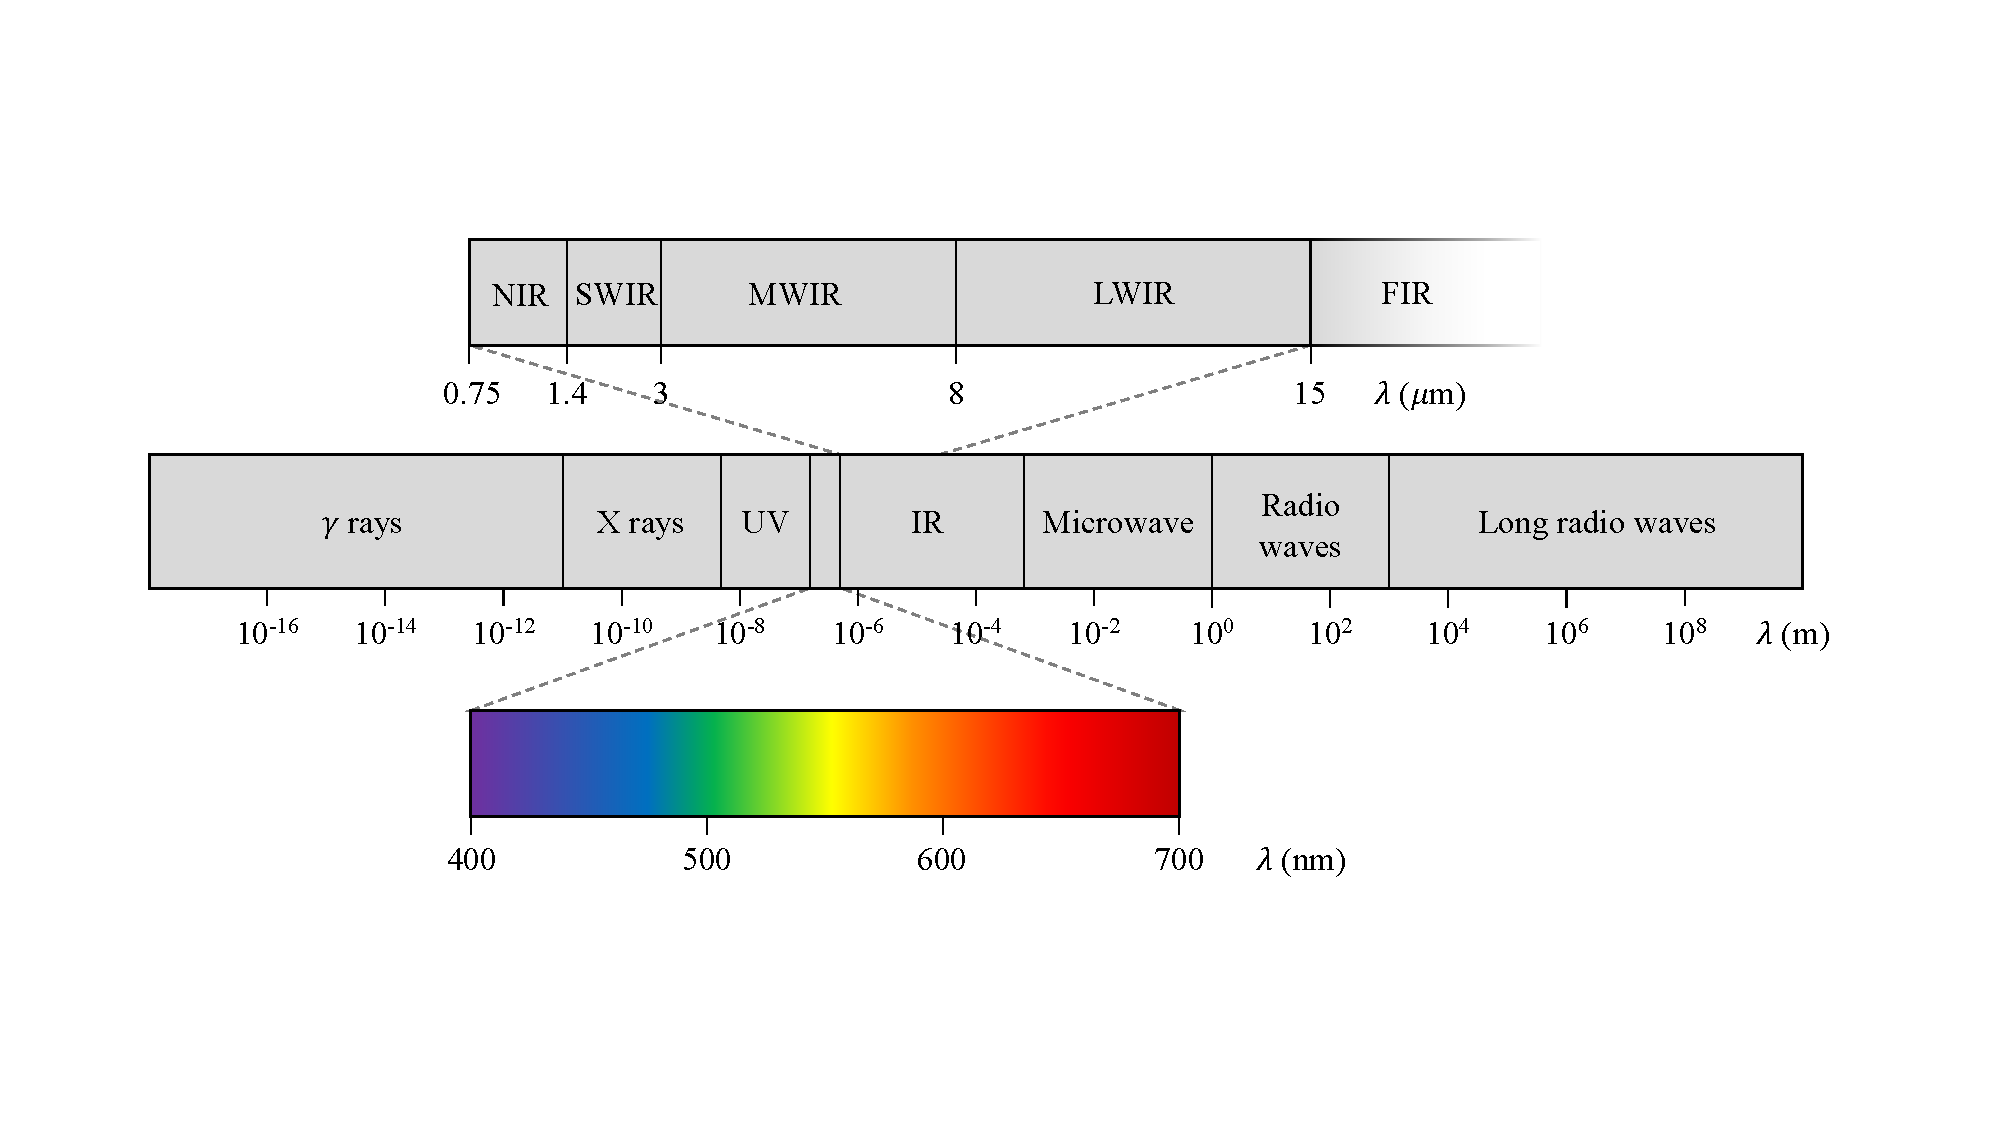
\includegraphics[width=\textwidth, trim={1.5cm 4cm 2cm 4cm}, clip=true]{images/EM_spectrum.pdf}
  \end{subfigure}
  \caption{The electromagnetic spectrum with detailled view of visible light and infrared. IR subdivisions modelled after \citet[p. 28]{byrnes_unexploded_2008}.}
  \label{fig:em_spectrum}
\end{figure}

\subsection{Thermal infrared radiation}

Black-body radiation is defined as thermal electromagnetic radiation emitted by an idealized opaque, non-reflective body \citep{young_sears_2012}. It has a continuous frequency spectrum that is dependent on the temperature of the body \citep{kogure_thermodynamic_2007}. The spectrum has a characteristic peak, which is inversely proportional to the temperature $T [K]$ according to Wien's displacement law:

\begin{equation}
  \lambda_{peak} = \frac{2.898 \times 10^{-3}}{T} [m],
\end{equation}

Bodies at a room temperature of $300 K$ emit electromagnetic radiation with a peak at $9.7 \mu m$ \citep{jarc_graz_2007}, falling into the LWIR range. To account for different non-ideal surfaces, the material-specific emissivity constant $\epsilon \in [0..1]$ is introduced to describe the share of radiation that is emitted by a body compared to an ideal black body. The total energy radiated by a body per unit surface and time is expressed by the Stefan-Boltzmann law:

\begin{equation}
  W = \epsilon \sigma T^4,
\end{equation}

where $\sigma$ is a proportionality constant. Thus, if the emissivity of a body is known, this law can be applied to determine its temperature based on the amount of LWIR-radiation received by a camera. This is the theoretical foundation for thermal imaging. 

In practice, the material and corresponding emissivity are often undetermined. Therefore, the received infrared radiation contains an unknown share of reflected radiation, adding noise to the measurement. This can be somewhat mitigated by estimating the value of $\epsilon$.

\subsection{Spectral imaging}

Spectral images combine spatial and spectral information in a 3-D data structure where the dimensions correspond to height, width and waveband. 
A distinction is made between hyperspectral and multispectral imaging techniques. 

If an image is acquired at many (tens or hundreds) regularly sampled wavebands, one speaks of a hyperspectral image, sometimes referred to as a hypercube. Hyperspectral images have many powerful applications, including agriculture and food quality \citep{dale_hyperspectral_2013} and medical applications \citep{lu_medical_2014}. However, capturing hyperspectral images requires advanced sensing equipment. Furthermore, hypercubes are difficult to process due to the high amount of information and, therefore, often require the application of computationally expensive preprocessing techniques, such as dimensionality-reduction \citep{qin_hyperspectral_2013}.

Multispectral images comprise of a few discrete wavebands. As opposed to hyperspectral images, it is usually not possible to extract a full continuous spectrum of an individual pixel from multispectral images \citep{abdul_multi-disnet_2019}. Whereas conventional visible-light cameras usually output images in the red, green, and blue channels (RGB), a multispectral system might comprise of additional wavebands, such as near infrared or long-wavelength infrared.


%----------------------------------------------------------------------------------------------------------------------------------

\section{Deep learning}

Deep learning is a branch of machine learning based on the concept of artificial neural networks (ANN). ANNs leverage the idea of artificial neurons, which are an abstract model derived from biological neurons. 

An artificial neuron consists of an input vector $\vec{x}$, a vector of weights $\vec{w}$, a bias $b$, an activation function $\varphi$, and an output scalar $y$. The input vector is multiplied with the weights element-wise. The sum of the result is computed and passed into the activation function, yielding the output. The output of an artificial neuron can, therefore, be computed as follows:

\begin{equation}
  y_j = \varphi (b + \sum_{i=0}^n x_i w_{ij}).
\end{equation}

Common choices for activation functions are sigmoid functions or rectified linear unit (ReLU), although various alternatives have been proposed \citep{ramachandran_searching_2017}.

In conventional ANNs, neurons are usually grouped into fully-connected layers. For each neuron in layer $j$, $\vec{x}$ represents the outputs of all neurons of the previous layer $j-1$. A traditional feed-forward neural network thus consists of an input layer, a sequence of multiple so-called hidden layers of artificial neurons, and an output layer. The behaviour of all neurons in a layer can be expressed as simple matrix multiplication, making it highly computationally efficient.

As proven by the universal approximation theorem, feed-forward neural networks can act as universal function approximators \citep{hornik_approximation_1991}. By defining a differentiable loss function for the output of the model, the coefficients of a neural network can be trained using the backpropagation algorithm \citep{rumelhart_learning_1986}. Backpropagation calculates the gradient of the loss function with respect to the weights of the layers in the model. Subsequently, it updates the weights following an optimisation algorithm such as gradient descent. This process is performed layer by layer, starting from the final layer of the network and moving backwards.

\subsection{Convolutional neural networks}

Convolutional neural networks (CNN) are a specialised type of neural network that makes use of convolution operations instead of general matrix multiplication for at least one of its layers \citep{goodfellow_deep_2016}. The 2-D discrete convolution, as commonly used in CNNs, is defined as follows:

\begin{equation}
  S(i, j) = (K \ast I) (i, j) = \sum_m \sum_n I(i-m, j-n) K(m, n),
\end{equation}

where $I$ denotes the $i \times j$ input tensor, $K$ is the $m \times n$ convolutional kernel (alternatively referred to as filter), and S is the $i \times j$ output or feature map. Depending on the kernel weights, convolution can be used for various image processing tasks, such as smoothing or edge detection.

\citet{lecun_backpropagation_1989} first used backpropagation to automatically learn the coefficients of convolutional filters as part of an image classification task. The kernels of a CNN are trained to recognise and aggregate important spatial features of an image. This is an advantage over fully-connected networks, as they are agnostic towards spatial relations of the input.

Convolutional layers in neural networks consist of multiple kernels that are applied to the input, usually resulting in an output tensor of depth equal to the number of filters. The amount of trainable coefficients of a convolutional layer is generally much lower than that of a fully-connected layer, making CNNs more computationally efficient. This enables the design of much deeper neural networks \citep{goodfellow_deep_2016}. CNNs with increasingly deep architectures have been shown to be highly effective on image classification and detection tasks, significantly outperforming conventional fully-connected networks \citep{krizhevsky_imagenet_2012, szegedy_going_2015, he_deep_2016}.


\subsection{Overfitting and dropout}

In practice, many machine learning models are good at correctly predicting training samples, but produce frequent errors when attempting to predict unknown samples. This property is called overfitting. Conversely, if the model performs poorly on both training and validation data, one speaks of underfitting. If a model is underfitted or overfitted, it is generally deemed to have low generalisability \citep{burkov_hundred-page_2019}. 

Due to the ability of neural networks with sufficient depth to approximate any multidimensional function, they are naturally susceptible to overfitting \citep{tetko_neural_1995}. It is, therefore, necessary to reduce the generalisation error of a deep learning model by employing strategies to combat overfitting. Such methods are known as regularisation techniques \citep{goodfellow_deep_2016}.

Dropout is a technique for addressing the problem of overfitting in ANNs that was introduced by \citet{srivastava_dropout_2014}. It attempts to reduce interdependent learning amongst neurons in a network. This is achieved by ignoring a random fraction of inputs to a given layer for each iteration during the training phase. A feature is ignored (dropped out) by setting it to 0.

Since nodes can not over-rely on specific inputs due to them being disabled during many training iterations, the network is forced to learn redundant connections. The model can learn more independent features, making it more robust. During the validation and prediction phase, no dropout is applied. Therefore, nodes are able to use all inputs for predictions.

Research has shown dropout to be highly effective for the regularisation of deep neural networks with fully-connected layers \citep{wu_towards_2015}. However, the effect of dropout on convolutional layers is still subject to active research. \citet{cai_effective_2019} state that traditional dropout is mostly ineffective on convolutional layers, creating training instability. They propose four alternative dropout methods (drop-neuron, drop-channel, drop-path and drop-layer) that have been explicitly designed for convolutional networks, reporting an increase in performance from all developed techniques. 

Many commonly used CNN designs, such as AlexNet \citep{krizhevsky_imagenet_2012}, include one or more fully-connected layers at the end to which dropout can be applied. 

\subsection{Standard evaluation techniques}

\subsubsection{Performance metrics}

Some of the most common performance metrics used to evaluate machine learning models are accuracy, precision, recall, and f1-score, which are defined as follows:

\begin{align}
  accuracy  &= \frac {TP + TN} {TP + TN + FP + FN}, \\
  precision &= \frac {TP} {TP + FP}, \\
  recall    &= \frac {TP} {TP + FN}, \\
  f1        &= \frac {2 \cdot precision \cdot recall} {precision + recall},
\end{align}

where TP is the number of true positives, FP is the number of false positives, TN is the number of true negatives, and FN is the number of false negatives. These metrics can be computed class-wise and aggregated across the whole dataset.

\subsubsection{Confusion matrix}

To visualise the classification errors generated by a supervised machine learning model, a confusion matrix can be created. Each row $i$ in the matrix corresponds to the instances of an actual class, whereas each column $j$ represents the instances of a predicted class. The value of each cell $i, j$ expresses the number of samples from class $i$ that were classified as class $j$. This makes it possible to inspect the confusion between different classes in the dataset.

%----------------------------------------------------------------------------------------------------------------------------------

\section{Recent developments and related work}

\subsection{Applications of thermal multispectral deep learning}

\subsubsection{Pedestrian detection}

One of the most actively researched applications for deep learning and thermal imaging is pedestrian detection. Autonomous systems such as self-driving cars need to be provided with accurate environmental information to guarantee safe operation. Traditional VIS-only models are often not able to provide this accuracy \citep{zhang_how_2016}, especially under challenging conditions such as insufficient illumination, partial object occlusion or weak contrasts between objects and background in the visible light spectrum. 

The KAIST Pedestrian Detection Benchmark \citep{hwang_multispectral_2015} was introduced to provide a prediction benchmark for thermal multispectral detection models. In recent years, many novel models and methodologies have been proposed, continuously improving the state of the art \citep{wagner_multispectral_2016, konig_fully_2017, guan_fusion_2019}.

\subsubsection{Facial recognition}

Another common application for deep learning and thermal imaging is facial recognition at low lighting conditions. The primary challenge of this task is matching thermal input images to a VIS-only database of faces \citep{choi_thermal_2012}. Proposed solutions include deep perceptual mappings (DPM) that aim to bridge the modality gap between visible-light and LWIR images \citep{sarfraz_deep_2017}. 

Commonly used datasets for multispectral facial recognition include Equinox \citep{selinger_appearance-based_2006} and the Laval University multispectral face database \citep{akhloufi_multispectral_2009}.

\subsubsection{Agriculture and food industry}

Furthermore, there are many applications of thermal imaging in agriculture and the food industry \citep{vadivambal_applications_2011}. Tasks such as food quality assessment and maturity evaluation can be automated using thermal imaging. For instance, \citet{gowen_applications_2010} reported the possibility to automatically detect bruised tissue on fruit and vegetables using thermal imaging. Based on a deep-learning approach, \citet{ibarra_combined_2000} proposed a noninvasive method for the estimation of the internal temperature of just-cooked meat. 

\subsubsection{Other applications}

\citet{lopez_detecting_2017} successfully developed a model for predicting exercise-induced fatigue for individuals. \citet{cho_deep_2018} introduced a novel technique for material type recognition using thermal imaging and deep learning. Their classifier can distinguish between 32 different materials. A model for estimating object distance based on multiple cameras, including thermal and visible light sensors, was proposed by \citet{abdul_multi-disnet_2019}.

\subsection{Architectures and techniques}

\citet{dollar_fast_2014} proposed a novel object detector based on aggregated channel features (ACF), achieving high object detection performance on visible-light images. This approach has been adapted to multispectral data, additionally incorporating the thermal channel T, and histograms of oriented gradients (HOG) features \citep{dalal_histograms_2005} extracted from the thermal channel. This model serves as a baseline for the KAIST dataset.

\citet{wagner_multispectral_2016} evaluated early and late feature fusion methods for thermal multispectral pedestrian detection. The early fusion approach involves stacking the RGB and T channels pixel-wise into a tensor of depth four and feeding the result into a CaffeNet \citep{jia_caffe_2014} convolutional network. The late fusion approach feeds the RGB image and LWIR image into separate convolutional networks respectively and merging the outputs using fully-connected layers. They concluded that, unlike the early fusion approach, the late fusion model significantly outperforms the previous state of the art ACF+T+HOG baseline. 

This model was further refined by \citet{osin_fast_2018} by evaluating different late fusion functions on a ResNet-based Single Shot MultiBox Detector (SSD) network \citep{liu_ssd_2016}. They achieved near real-time detection performance on embedded systems.

Expanding upon the late fusion network introduced by \citet{wagner_multispectral_2016}, \citet{guan_fusion_2019} proposed an illumination-aware approach to multispectral deep learning models. This approach is based on two-stream networks, as introduced by \citet{simonyan_two-stream_2014}. After the outputs of the RGB and LWIR networks are fused, they are fed into separate networks for daytime and nighttime images. The respective predictions are then merged using illumination-aware weights. This approach achieved state-of-the-art performance on the KAIST benchmark.

\citet{wu_intraspectrum_2020} developed an approach for face recognition based on a novel spectrum pooling layer. The channels of the input image are passed into individual CNNs. The spectrum pooling layer subsequently selects the outputs of the CNNs with the strongest discriminative abilities. The selected features are then passed into a fully-connected layer. This approach achieves superior performance for several face recognition datasets.

%==================================================================================================================================

\chapter{Problem analysis}
\label{analysis}

\section{Data acquisition}

Collecting a multispectral dataset of sufficient quality is significantly more challenging than a dataset consisting solely of visible-light images. Specialised equipment is needed to obtain samples. Using two sensors to capture the different channels introduces problems such as channel misalignment and inability to perform an optical zoom. This makes it harder to frame the objects of interest properly.

Furthermore, most image classification tasks use traditional visible-light imaging only. As a result, the research and resources that are available for use are much more limited.

\subsection{Sensory equipment}
\label{sensory_equipment}

Even though thermal cameras have become significantly more affordable in recent years, their resolution remains much lower than that of conventional visible-light cameras. The FLIR One Pro \footnote{\url{https://www.flir.com/products/flir-one-pro/}}, which was used for this project, is composed of two sensors:

\begin{itemize}
  \item A conventional camera for visible-light images with a resolution of $1440 \times 1080$ px.
  \item A thermal sensor with a spatial resolution of $160 \times 120$ px and a spectral range of $8 - 14 \mu m$.
\end{itemize}

The FLIR camera is, therefore, able to perceive and record electromagnetic waves in the visible-light (VIS) and long-wave infrared (LWIR) bands. Furthermore, images can be captured at a frequency of $8.7 Hz$, enabling real-time vision. Due to technical limitations, several challenges had to be overcome when working with data collected by the sensor.

Firstly, the two cameras are not spatially aligned. Furthermore, the "zoom level" or focal length of the sensors does not appear to match. A misalignment of the channels is likely to have an adverse impact on the performance of a convolutional network \citep{chappelow_improving_2008}. Therefore, the issue of image registration of the two camera outputs arises. The strategy we introduced to perform robust registration of the VIS and LWIR images is outlined in Section \ref{image_registration}.

Secondly, the different resolutions of the sensors could cause problems too, as convolutional filters might struggle to detect edges and other features consistently across all channels. A possible strategy to avoid this issue is to resize the images to a common resolution. However, this means that valuable information in the VIS image might be lost and overall accuracy might be reduced. It is, therefore, necessary to evaluate the degree of information loss upon size reduction of the visible-light image.

%----------------------------------------------------------------------------------------------------------------------------------

\section{Modality gap between LWIR and VIS images}
\label{modality}

As outlined in Section \ref{imaging}, LWIR and visible light are both forms of electromagnetic radiation. However, the properties of LWIR and VIS images differ significantly. \citet{sarfraz_deep_2017} refer to visible light as reflection-dominant and LWIR as emission-dominant radiation, resulting in a modality gap between the two corresponding sensing techniques. \citet{choi_thermal_2012} consider this modality gap a challenging problem for computer vision algorithms.

\citet{davis_background-subtraction_2007} state that thermal cameras are especially effective for object detection tasks compared to VIS cameras in low-light settings. Conversely, given sufficient illumination, visible-light cameras perform better than thermal sensors if the thermal properties of objects are similar to their background. Furthermore, they state a low signal-to-noise ratio and white-black polarity calibration issues as common problems of thermal cameras.

\subsection{Textural features}

To evaluate the different textural properties of thermal and visible-light images, a test image was taken in an indoor setting. The LWIR channel and the greyscale representation of the RBG channels can be seen in Figures \ref{fig:fourier_lwir_spatial} and \ref{fig:fourier_vis_spatial}. It is apparent that the greyscale image contains more textural details than the LWIR image. For instance, the painting above the fireplace appears as a simple gradient in the thermal band.

\begin{figure}[ht]
  \centering
  \begin{subfigure}[h!]{0.4\textwidth}
    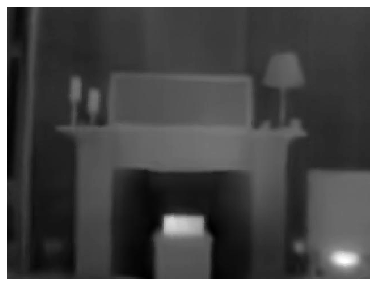
\includegraphics[width=\textwidth]{images/fourier/lwir_spatial}
    \caption{LWIR spatial domain}
    \label{fig:fourier_lwir_spatial}
  \end{subfigure}
  \begin{subfigure}[h!]{0.4\textwidth}
    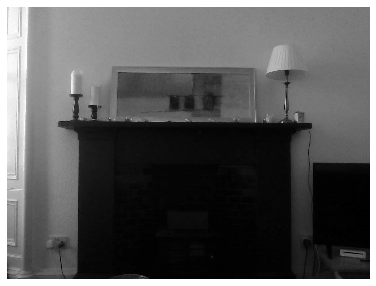
\includegraphics[width=\textwidth]{images/fourier/gray_spatial}
    \caption{VIS spatial domain}
    \label{fig:fourier_vis_spatial}
  \end{subfigure}
  \begin{subfigure}[h!]{0.4\textwidth}
    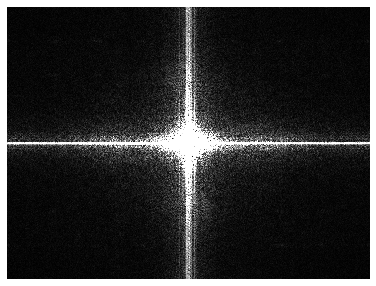
\includegraphics[width=\textwidth]{images/fourier/lwir_freq}
    \caption{LWIR frequency domain magnitude}
    \label{fig:fourier_lwir_freq}
  \end{subfigure}
  \begin{subfigure}[h!]{0.4\textwidth}
      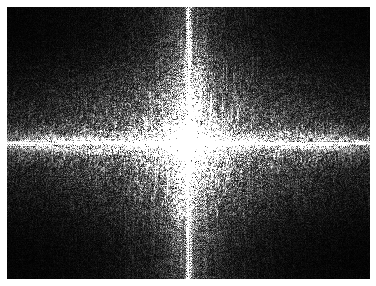
\includegraphics[width=\textwidth]{images/fourier/gray_freq}
      \caption{VIS frequency domain magnitude}
      \label{fig:fourier_vis_freq}
    \end{subfigure}
  \caption{Fast discrete Fourier transform of an example LWIR and VIS image. The VIS image contains more detailed textural information, making it \textit{noisier}, as can be seen in the frequency domain.}
  \label{fig:fourier}
\end{figure}

We applied a fast Fourier transform \citep{cooley_fast_1969} to both images. Fourier transforms are a method for decomposing a signal into its sinusoidal components. The original image is considered to be in the spatial domain, whereas the transformed signal represents the same information in the frequency domain. It consists of the two complex components magnitude and phase. In this case, translating into the frequency domain allows the analysis and modification of the image's geometric structure. 

Figures \ref{fig:fourier_lwir_freq} and \ref{fig:fourier_vis_freq} show the magnitude component of the aforementioned image in the frequency domain. The centre has been shifted to represent the zero frequency of the image. The distance of a point to the centre represents its frequency and the intensity its magnitude. 

It can be seen that the visible-light image has a significantly higher portion of high-frequency components than its LWIR counterpart. Hence, the VIS image can be considered to be noisier than the LWIR image. This effect does not change significantly when downsampling the VIS image to the resolution of $160 \times 120$. The difference in texture details might have an impact on the effects of convolutional filters on the LWIR and VIS images.

\subsection{Environmental conditions}

Figure \ref{fig:fourier}, furthermore, demonstrates the strengths and weaknesses of both types of sensors. Due to insufficient lighting, the whole fireplace appears as a single almost completely black surface in the VIS image. The LWIR image clearly shows two objects standing in front of the fireplace. On the other hand, the thermal image does not capture many details visible in the VIS image, such as the texture of the painting.

Hence, it appears as if a benefit of LWIR cameras compared to visible light can be achieved mainly in scenarios with a high thermal contrast and adverse lighting conditions. Most mammals and avian species actively regulate their internal temperature \citep{prinzinger_body_1991} and can be picked up easily by a thermal camera. Therefore, it can be theorised that the classification of animals could be significantly improved using a thermal multispectral sensing technique.

Due to limited access to the animals, a robust evaluation of the relative performance of a multispectral model in different lighting conditions was not performed as part of this project.

%----------------------------------------------------------------------------------------------------------------------------------

\section{Transfer learning}
\label{transfer_learning_analysis}

A large amount of existing datasets is available for traditional image classification tasks. The ImageNet dataset \citep{deng_imagenet_2009}, which is used as a benchmark for many image classification models, contains over a million labelled images that can be used to train a model. Many successful deep learning models, such as AlexNet \citep{krizhevsky_imagenet_2012} and ResNet \citep{he_deep_2016} have been applied to datasets such as ImageNet.

When creating an image classifier for a new application, it is then possible to make use of a model that has been pre-trained on another dataset, such as ImageNet. This model can subsequently be adapted to the new data by exchanging the final fully-connected layer of that network for one that suits the new classification task. Finally, the model can be trained on the new dataset. This strategy is known as transfer learning and was introduced by \citet{thrun_is_1996}.

Since the features learned by early layers are often applicable across many classes and images (e.g. edge or texture features), the network generalises better, as it has been trained on an overall larger dataset. Therefore, transfer learning makes it feasible to train complex models on smaller amounts of data than usual \citep{kwasniewska_deep_2017}.

For multispectral models, this highly effective approach becomes more difficult, as much fewer datasets are available to be used off-the-shelf. Datasets for visible light and thermal data, such as the KAIST Pedestrian Detection Benchmark \citep{hwang_multispectral_2015} are available. However, They usually lack the number of classes and the overall size of traditional computer vision datasets and are, therefore, less suitable for transfer learning tasks.

Pre-training a multispectral classifier on a VIS-only dataset is not directly possible due to the incompatible input tensor shapes ($h \times w \times 3$ compared to $h \times w \times 4$) and the resulting difference in trainable weights. Moreover, the modality gap outlined in Section \ref{modality} makes it likely that this approach would be unfeasible even if the tensor shapes were compatible.

However, there are strategies to mitigate this issue. It is possible to divide the model into two separate branches of layers that process the VIS and LWIR images individually, and perform late feature-level fusion \citep{wagner_multispectral_2016, guo_face_2017} by concatenating the respective feature maps and adding at least one fully connected layer after the concatenation. This approach can make it possible to load pre-trained weights into the VIS-branch of the model without affecting the LWIR branch. During training, the LWIR-branch of the model gets trained from scratch, whereas transfer learning is simultaneously performed on the VIS-branch.

Another possible approach to enable the usage of existing off-the-shelf datasets is to perform generative image augmentation. In Section \ref{autoencoder_implementation}, we explore the application of a primitive generative model for predicting the corresponding LWIR image of a known type of object from a given RGB image. Given sufficient quality of predicted images, it would then be possible to turn RGB-only images into multispectral training data.

%----------------------------------------------------------------------------------------------------------------------------------

\section{Mobile application}
\label{analysis_mobile_application}

This project aimed to deploy the final deep learning model to a mobile edge device. This introduced many challenges related to mobile computing. Contrary to most computers, computational power on mobile devices is highly limited. Furthermore, to provide robust and reliable real-time classification, low latency between image capture and classification was necessary. Two major strategies can be used to perform image classification on a mobile device:

\begin{enumerate}
  \item Deploy the model to a web service, upload captured frames from the edge device, and retrieve the prediction. This requires minimal computational power on the edge device, as all calculations are performed remotely. However, it might come at the cost of increased latency from transmitting the input images to the server. Furthermore, in situations with poor connectivity, such as remote regions, no classification can be performed.
  \item Deploy the model to the edge device and perform all computations \textit{offline} on the mobile device. This avoids potential connectivity problems while requiring sufficient computational efficiency to be able to run in real-time.
\end{enumerate}

Whereas the latter approach appears more robust than the prior one, it introduces a variety of problems. The amount of deep learning and image processing tools available for Java and Android is limited compared to the Python machine learning stack. Libraries such as TensorFlow only provide simplified APIs with reduced functionality for Java. Many image processing libraries do not support multispectral data, further complicating image processing.


%==================================================================================================================================

\chapter{Design}
\label{design}

\section{Dataset}

\subsection{Classes and samples}
\label{classes_samples}

Initially, a dataset consisting of 13 classes and 1042 samples was captured at Tollcross Children's Farm, Glasgow using the camera functionality of the mobile application. Similarly to a video, the app captures images in quick temporal succession. Thus, many samples are relatively similar, as they were taken within only a few milliseconds difference. To distinguish between different bursts of images, samples were grouped into distinct subsets, each subset representing a batch of similar samples.

Due to the difficulty of obtaining well-framed and unobstructed images, the data contains significant noise. Some images contain more than one animal. Furthermore, some animals were housed in closed-off shelters and were only visible behind a metal grid. This is problematic, as a classifier is likely to learn the various obstructions as features of specific classes. This can negatively impact generalisability, as the model might not be able to predict unobstructed images of these classes correctly.

Therefore, each subset was labeled as either \textit{single}, \textit{multi} or \textit{obstructed} to allow greater flexibility when selecting data for training and validation. Moreover, no distinction between genders was made. Multiple colour variations of alpacas and chickens are represented in the dataset.

\begin{table}[ht]
  \centering
  \begin{tabular}{@{}llll@{}}
    \toprule
    \textbf{Class}  & \textbf{Dataset 1} & \textbf{Dataset 2} & \textbf{Dataset 3}  \\ \midrule
    Cat             & 205              & 0                    & 0                   \\ 
    Pig             & 30               & 0                    & 0                   \\
    Pony            & 112              & 127                  & 234                 \\
    Sheep           & 36               & 0                    & 0                   \\
    Alpaca          & 85               & 391                  & 115                 \\
    Ferret          & 33               & 0                    & 0                   \\
    Peacock         & 157              & 79                   & 0                   \\
    Hamburg chicken & 29               & 58                   & 49                  \\
    Silkie chicken  & 17               & 129                  & 83                  \\
    Muscovy duck    & 24               & 141                  & 105                 \\
    Chicken         & 138              & 151                  & 170                 \\
    Rabbit          & 32               & 16                   & 0                   \\
    Goose           & 144              & 0                    & 0                   \\ \bottomrule
  \end{tabular}
  \caption{Classes and sample size of raw animals datasets.}
  \label{table:raw_dataset}
\end{table}

Initially, the separation into training and validation data was performed using a stratified random split of all the data. As demonstrated in Section \ref{eval_train_val_split}, nearly perfect validation accuracy was achieved on this split. This is most likely a result of the aforementioned similarity of many images due to them being captured at similar times. Hence, we decided that a second independent dataset was necessary to achieve representative evaluation results. Two more datasets were captured on different days to obtain a wider range of lighting situations and background scenarios. The classes and samples of all three datasets are shown in Table \ref{table:raw_dataset}.

Finally, the subsets from the raw datasets were rearranged into a training dataset and a validation dataset. To avoid the issue of fitting and validating on similar images, each subset was assigned to one of the two datasets. An attempt was made to obtain a balanced mixture of \textit{single}, \textit{multi}, and \textit{obstructed} subsets in both datasets. Furthermore, subsets that were deemed too noisy were omitted. Nonetheless, it can be assumed that achieving a perfect and representative split is difficult due to the noise in the dataset and the limited variety of contexts. The final train-validation-split is shown in Table \ref{table:train_test_dataset}. Overall, 35 subsets were assigned to the training dataset, and 19 were allocated to the validation dataset.

\begin{table}[ht]
  \centering
  \begin{tabular}{@{}lll@{}}
    \toprule
    \textbf{Class}  & \textbf{Train (subsets)} & \textbf{Validation (subsets)} \\ \midrule
    Cat             & 149 (3)                  & 56  (1)        \\
    Pony            & 415 (5)                  & 58  (4)        \\
    Alpaca          & 377 (4)                  & 87  (2)        \\
    Hamburg chicken & 77  (3)                  & 59  (3)        \\
    Silkie chicken  & 191 (3)                  & 38  (2)        \\
    Muscovy duck    & 206 (6)                  & 64  (4)        \\
    Chicken         & 277 (10)                 & 119 (2)        \\
    Goose           & 125 (1)                  & 19  (1)        \\ \bottomrule
  \end{tabular}
  \caption{Sample size and subset composition of train and validation datasets.}
  \label{table:train_test_dataset}
\end{table}

The classes with low support (Pig, Sheep, Ferret, Rabbit) were dropped from the datasets, as it was deemed unlikely that a model would be able to generalise well on such small numbers of samples. Moreover, it was not possible to capture pictures of peacocks from a sufficient variety of contexts. Instead of training and validating on similar images of peacocks, the class was removed from the datasets. A problem that remained is the class imbalance in both datasets. Alpacas and ponies are over-represented, and Hamburg chickens are significantly under-represented.

\begin{figure}[ht]
  \centering
  \begin{subfigure}[h!]{0.18\textwidth}
    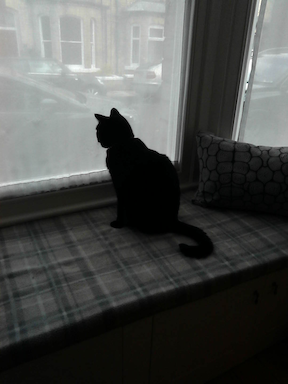
\includegraphics[width=\textwidth, trim={0cm 2.5cm 0cm 2.5cm}, clip]{images/dataset/cat/rgb.png}
    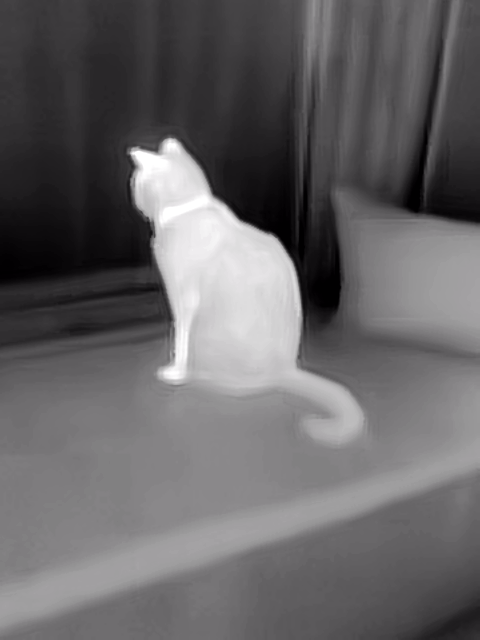
\includegraphics[width=\textwidth, trim={0cm 2.5cm 0cm 2.5cm}, clip]{images/dataset/cat/lwir.png}
    \caption{Cat}
  \end{subfigure}
  \begin{subfigure}[h!]{0.18\textwidth}
    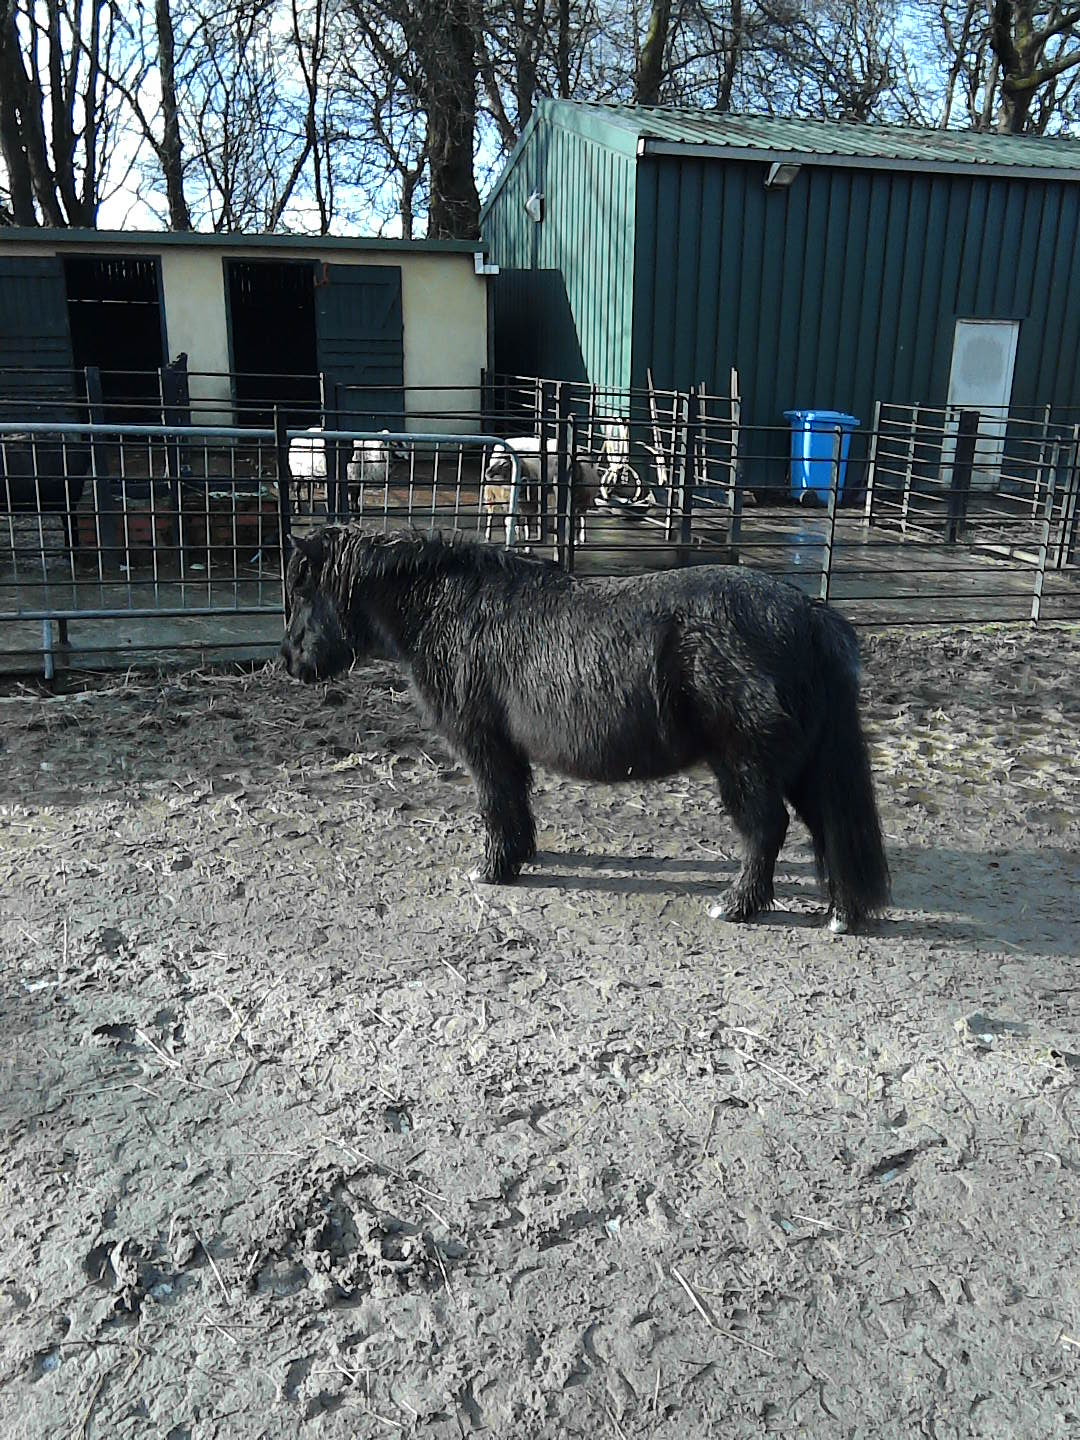
\includegraphics[width=\textwidth, trim={0cm 2.5cm 0cm 2.5cm}, clip]{images/dataset/pony/rgb.png}
    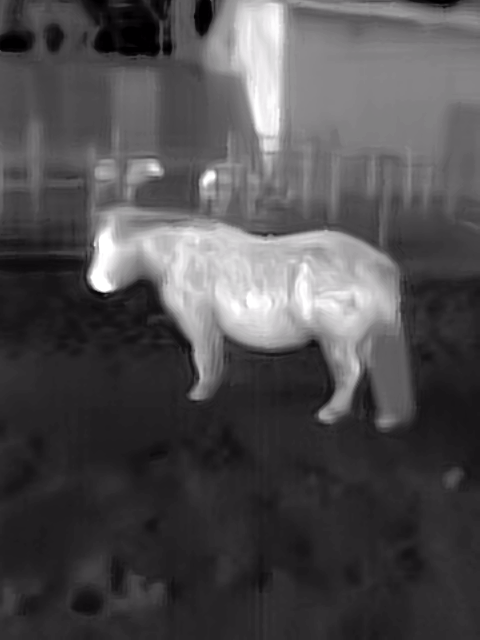
\includegraphics[width=\textwidth, trim={0cm 2.5cm 0cm 2.5cm}, clip]{images/dataset/pony/lwir.png}
    \caption{Pony}
  \end{subfigure}
  \begin{subfigure}[h!]{0.18\textwidth}
    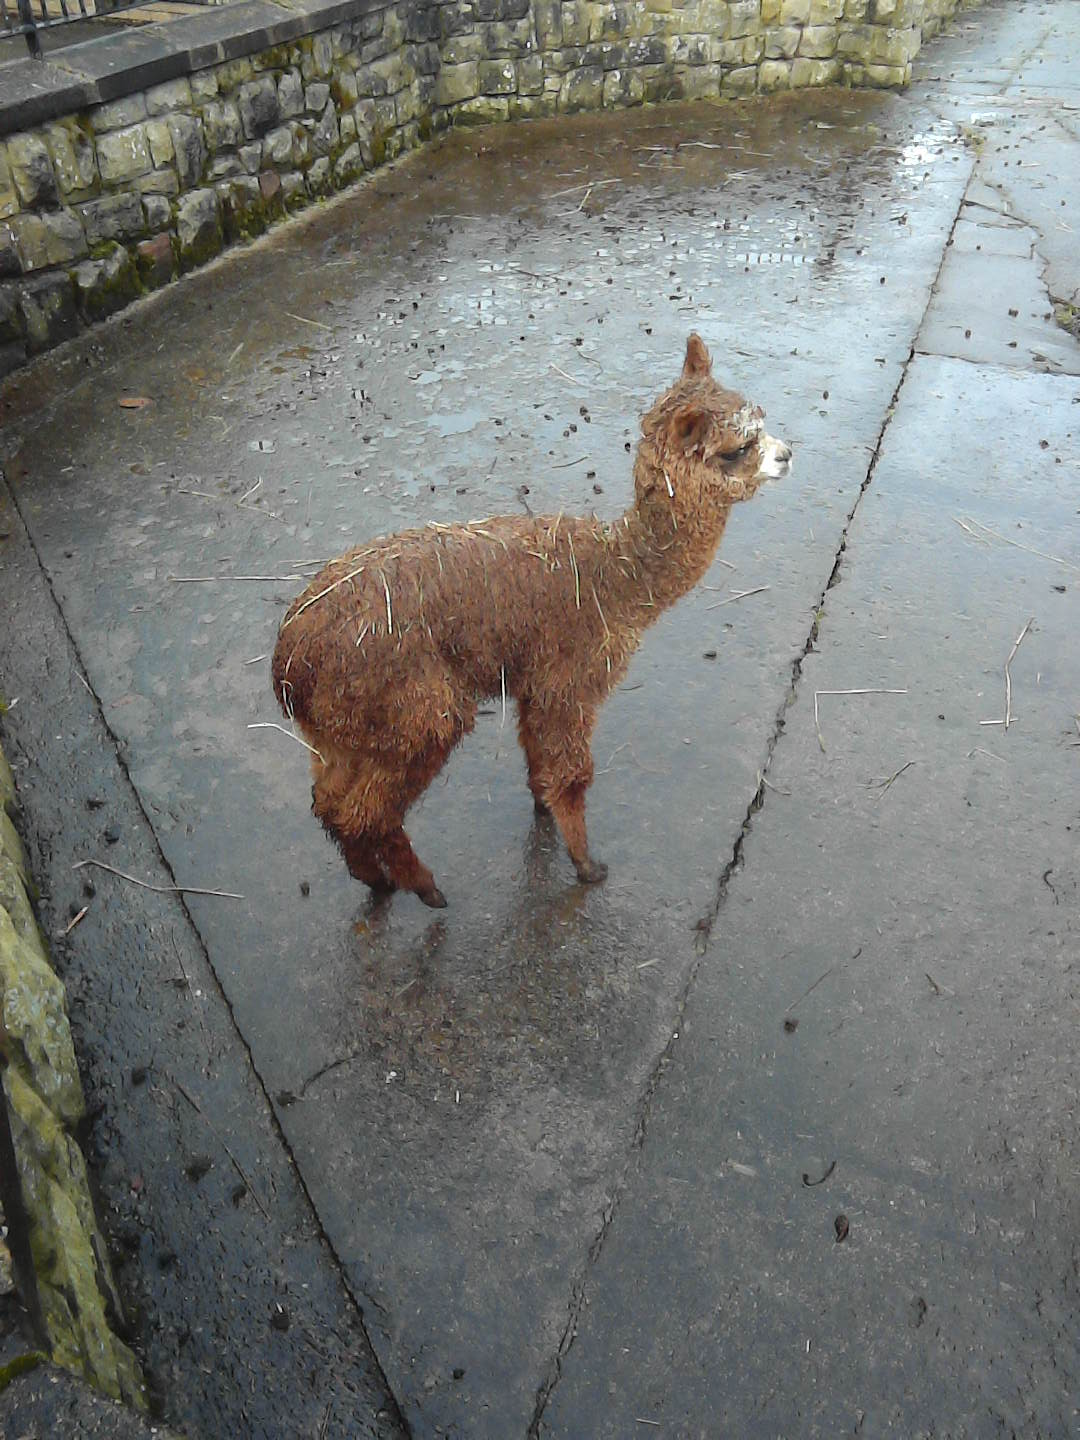
\includegraphics[width=\textwidth, trim={0cm 2.5cm 0cm 2.5cm}, clip]{images/dataset/alpaca/rgb.png}
    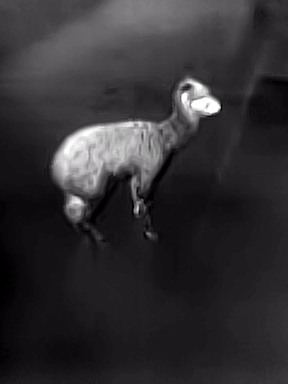
\includegraphics[width=\textwidth, trim={0cm 2.5cm 0cm 2.5cm}, clip]{images/dataset/alpaca/lwir.png}
    \caption{Alpaca}
  \end{subfigure}
  \begin{subfigure}[h!]{0.18\textwidth}
    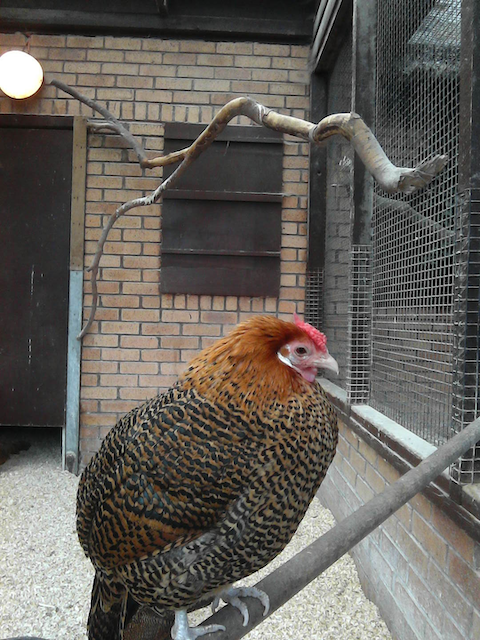
\includegraphics[width=\textwidth, trim={0cm 2.5cm 0cm 2.5cm}, clip]{images/dataset/pretty_chicken/rgb.png}
    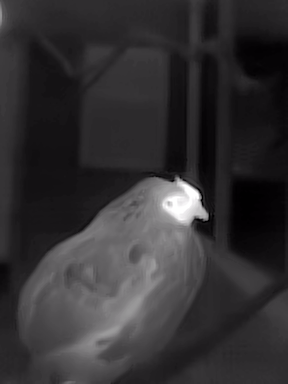
\includegraphics[width=\textwidth, trim={0cm 2.5cm 0cm 2.5cm}, clip]{images/dataset/pretty_chicken/lwir.png}
    \caption{Hamburg chicken}
  \end{subfigure}
  \\
  \begin{subfigure}[h!]{0.18\textwidth}
    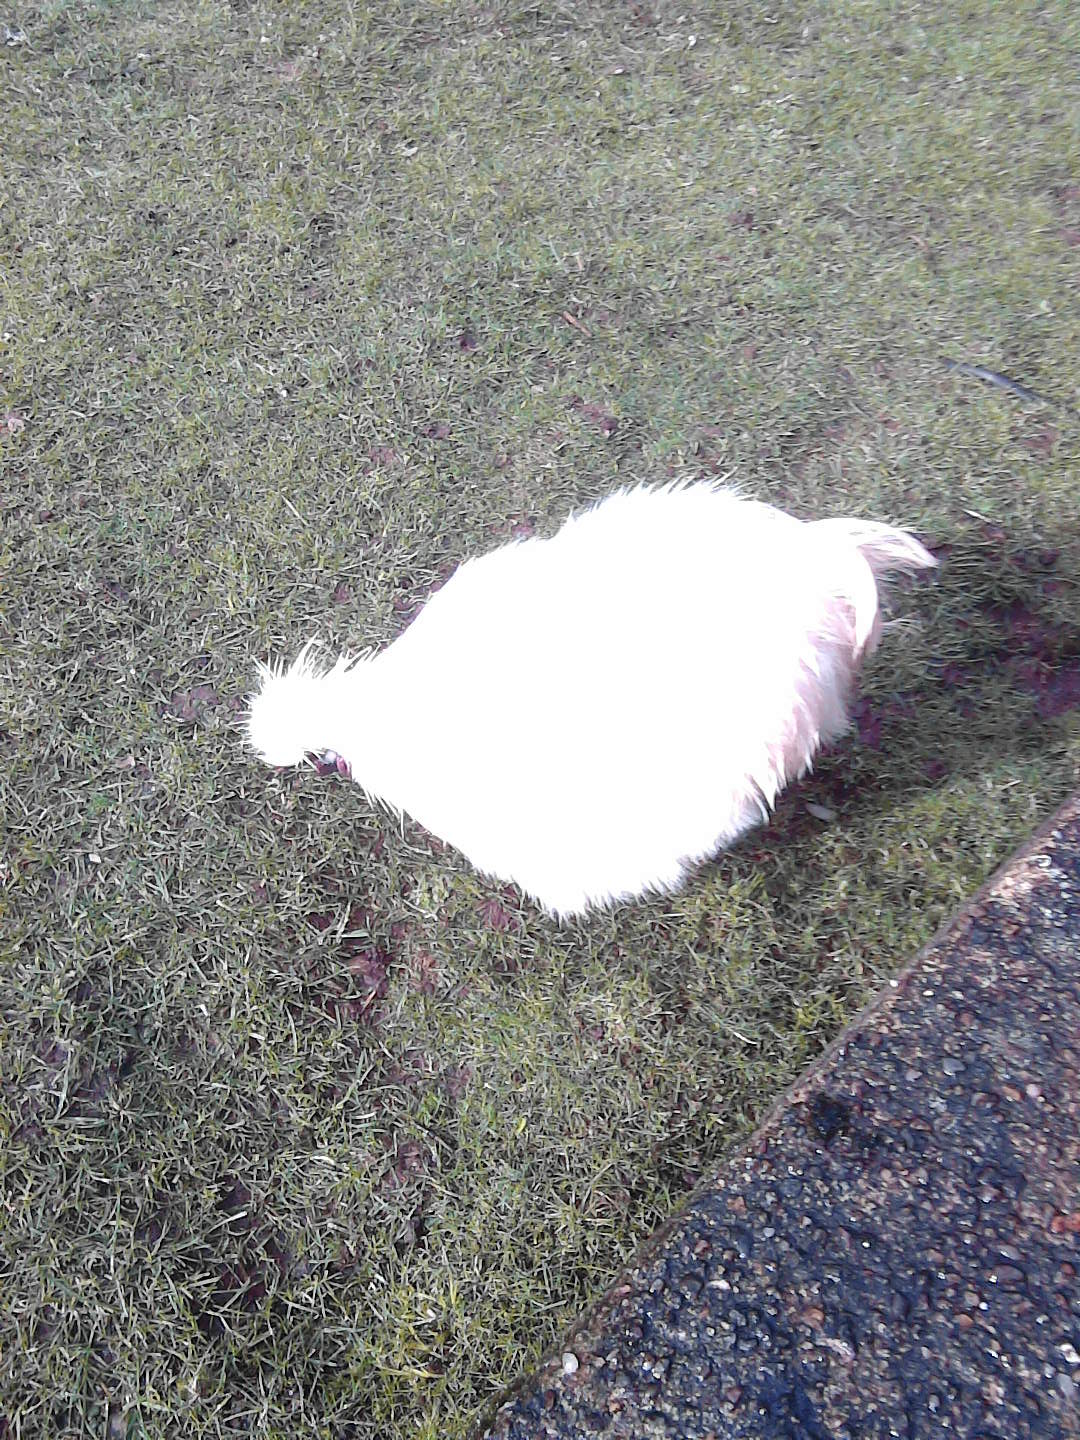
\includegraphics[width=\textwidth, trim={0cm 2.5cm 0cm 2.5cm}, clip]{images/dataset/evil_chicken/rgb.png}
    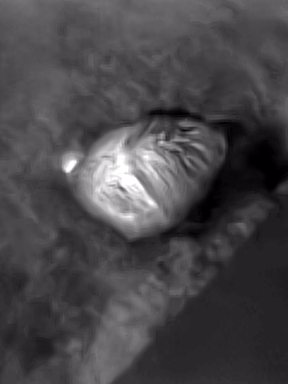
\includegraphics[width=\textwidth, trim={0cm 2.5cm 0cm 2.5cm}, clip]{images/dataset/evil_chicken/lwir.png}
    \caption{Silkie chicken}
  \end{subfigure}
  \begin{subfigure}[h!]{0.18\textwidth}
    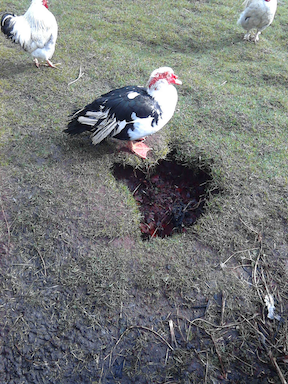
\includegraphics[width=\textwidth, trim={0cm 2.5cm 0cm 2.5cm}, clip]{images/dataset/ugly_duck/rgb.png}
    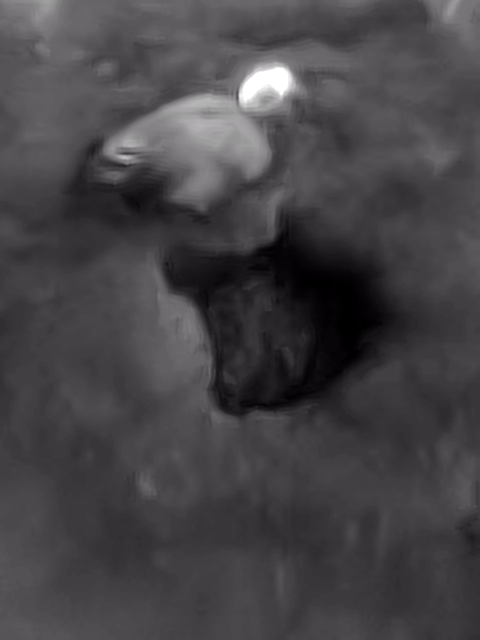
\includegraphics[width=\textwidth, trim={0cm 2.5cm 0cm 2.5cm}, clip]{images/dataset/ugly_duck/lwir.png}
    \caption{Muscovy duck}
  \end{subfigure}
  \begin{subfigure}[h!]{0.18\textwidth}
    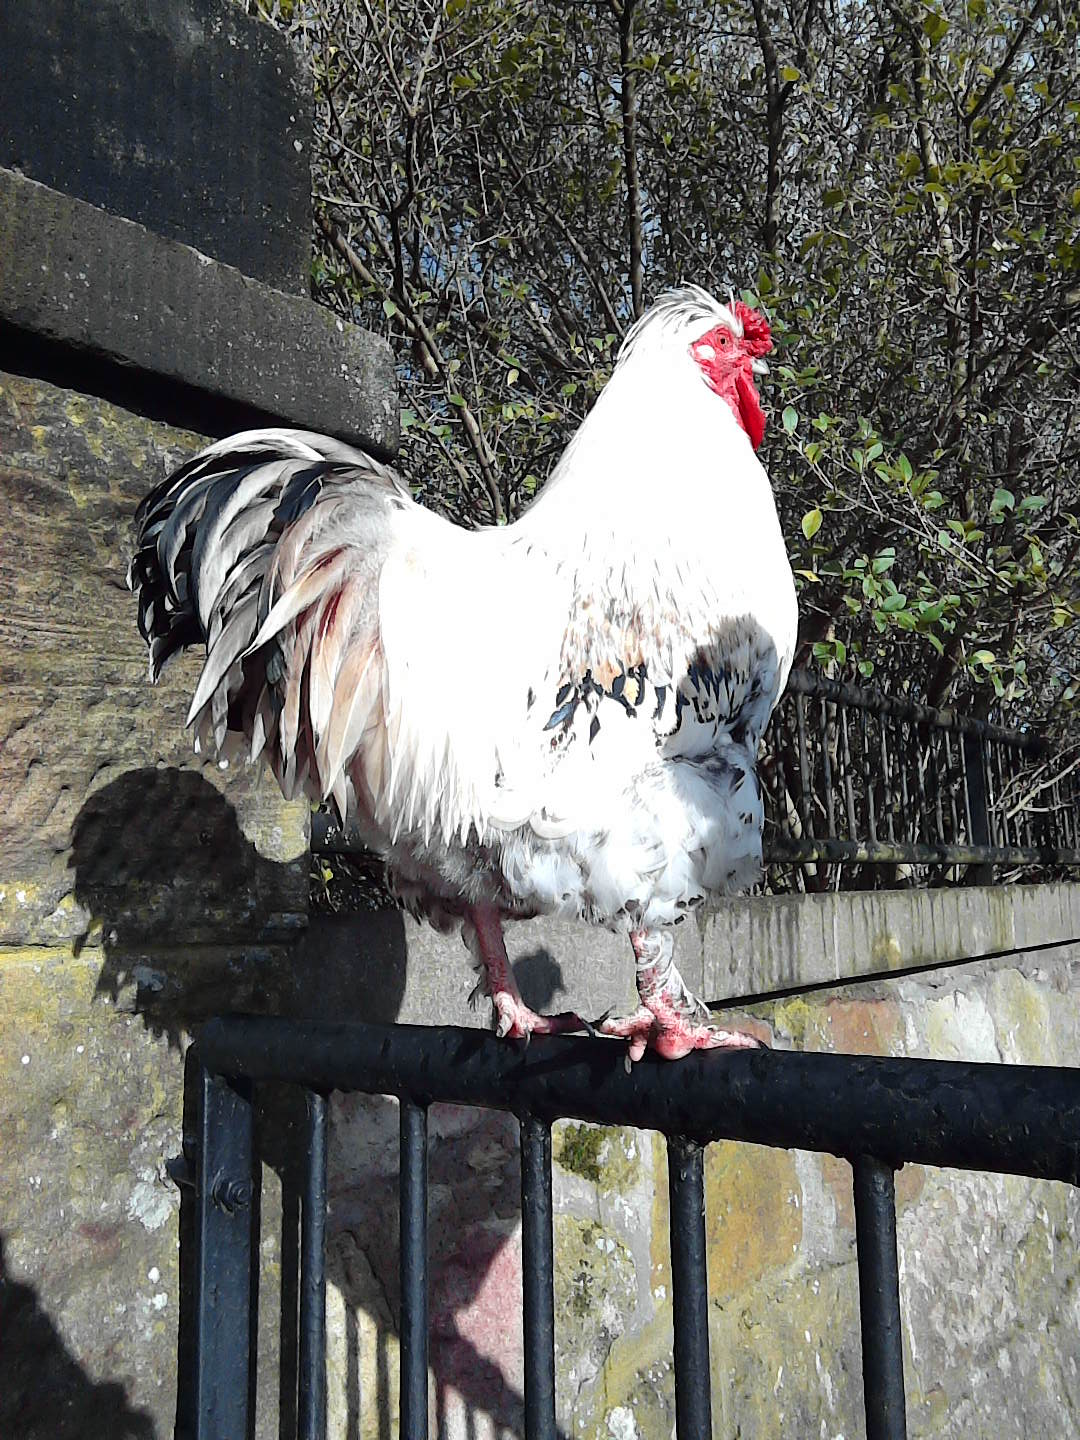
\includegraphics[width=\textwidth, trim={0cm 2.5cm 0cm 2.5cm}, clip]{images/dataset/chicken/rgb.png}
    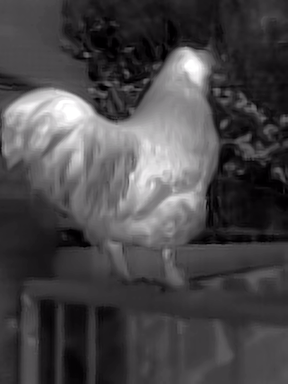
\includegraphics[width=\textwidth, trim={0cm 2.5cm 0cm 2.5cm}, clip]{images/dataset/chicken/lwir.png}
    \caption{Chicken}
  \end{subfigure}
  \begin{subfigure}[h!]{0.18\textwidth}
    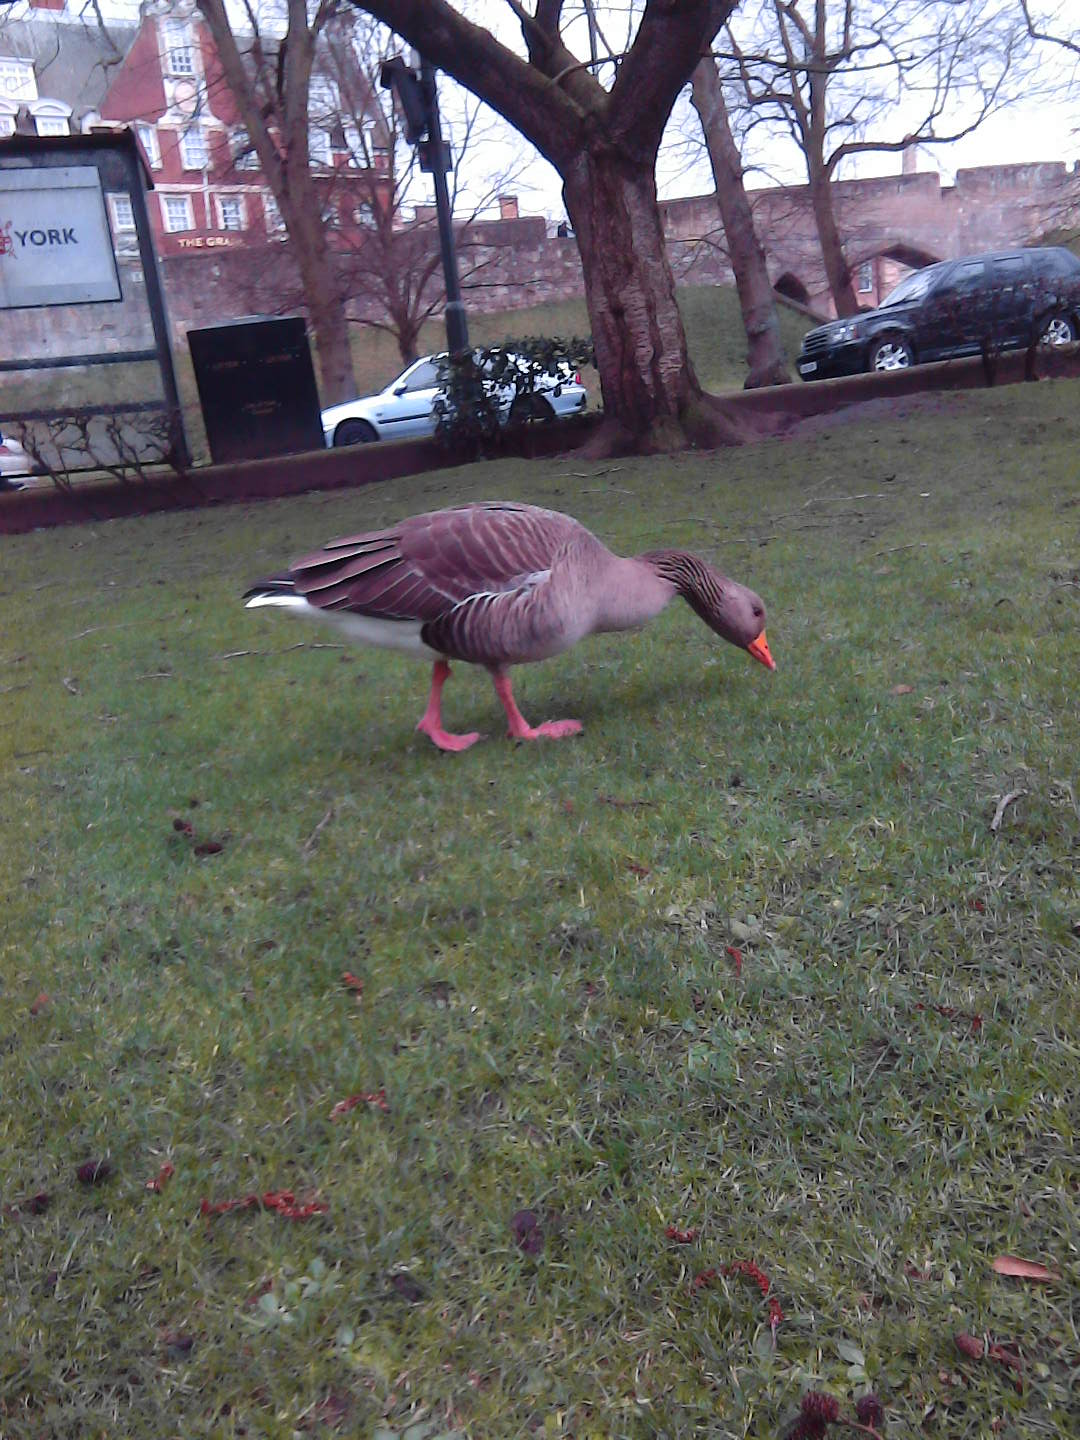
\includegraphics[width=\textwidth, trim={0cm 2.5cm 0cm 2.5cm}, clip]{images/dataset/goose/rgb.png}
    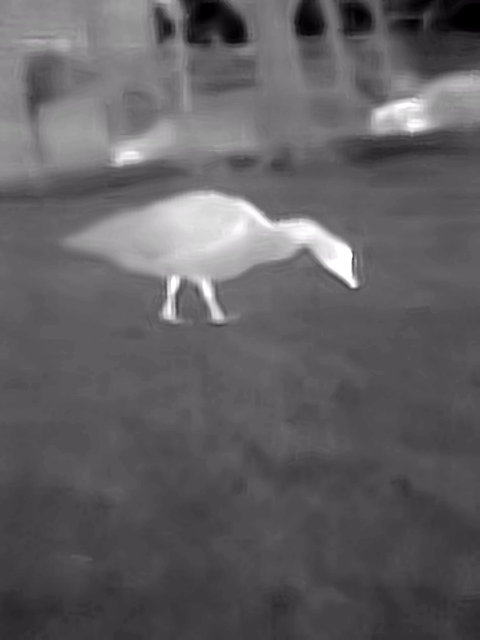
\includegraphics[width=\textwidth, trim={0cm 2.5cm 0cm 2.5cm}, clip]{images/dataset/goose/lwir.png}
    \caption{Goose}
  \end{subfigure}
  \caption{Example images for each class in the final dataset. Images have been cropped vertically.}
  \label{fig:dataset_classes}
\end{figure}

Figure \ref{fig:dataset_classes} shows example VIS and LWIR images from the training dataset. While these examples are sampled from the idealised \textit{single} subsets without obstructions, they highlight another critical caveat. Not all images could be captured at the same distance. Consequently, different animals fill different amounts of space within the images, possibly skewing classification results. An attempt was made to mitigate this issue through affine data augmentation.

\subsection{Data augmentation}

Due to the limited amount of time and resources available to the project, generating a dataset with sufficient scope and size proved to be challenging. Since the performance of machine learning models is usually directly tied to the size and quality of the available dataset, an insufficient dataset can make it impossible to train an accurate and robust classifier \citep{fawzi_adaptive_2016}. Therefore, data augmentation was employed to increase the number of usable training samples artificially.

\citet{mikolajczyk_data_2018} made the distinction between white-box and black-box data augmentation methods. While the latter use a form of deep learning known as Generative Adversarial Networks (GAN) to synthesise new training samples, white-box methods involve more traditional techniques, such as affine transformations. An affine transformation or affine map can accurately represent a composition of a translation and a linear map (e.g. scaling, rotation and shearing). A transformation $f(\vec{x})$ can be expressed as follows:

\begin{equation}
  f(\vec{x}) = A \vec{x} + \vec{b},
  \label{eqn:affine}
\end{equation}

where $\vec{x}$ represents the coordinates of a point to be translated, $A$ is a $2 \times 2$ linear map, and $\vec{b}$ is the translation vector. $f(\vec{x})$ can be applied to the coordinates $\vec{x}$ of every pixel, yielding a transformed image. If necessary, interpolation strategies are used to fill in gaps between the new pixels.

After evaluating various methods of data augmentation on a subset of the ImageNet dataset, \citet{perez_effectiveness_2017} concluded that traditional affine transformations alone can be effective at improving classification performance, although GAN-based methods are promising and might yield better results.

Due to the relatively easy implementation, this project made heavy use of white-box data augmentation. However, the design and implementation of a deep convolutional autoencoder for generating LWIR from visible-light images is discussed in Section \ref{autoencoder_implementation}. This model could be used to generate new LWIR data samples from visible-light images retrieved from other sources, such as existing VIS-only image classification datasets.

Figure \ref{fig:augmentation_affine} shows different affine transformations that were used to augment the captured dataset. The most natural transformation in this scenario is a horizontal flip, as we can assume that the objects to be classified are symmetric along the horizontal axis, and the images have all been captured with similar camera orientations. Moreover, we employed randomized zooms to try to account for the varying distances at which the animals were photographed. We decided to limit the zoom factor to a small enough range to guarantee that the images still showed the whole object. Finally, we applied random rotations in the range from $-20^{\circ}$ to $20^{\circ}$ to account for slightly different camera orientations.

\begin{figure}[ht]
  \centering
  \begin{subfigure}[h!]{0.24\textwidth}
    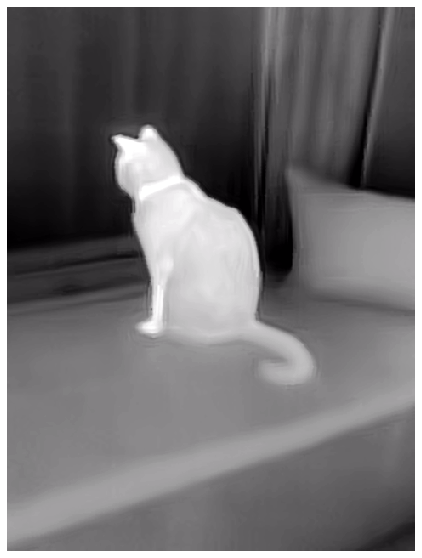
\includegraphics[width=\textwidth]{images/augmentation/original.png}
    \caption{Original image}
  \end{subfigure}
  \begin{subfigure}[h!]{0.24\textwidth}
    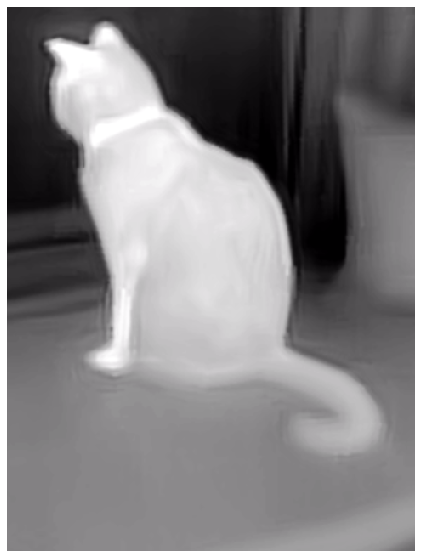
\includegraphics[width=\textwidth]{images/augmentation/zoomed.png}
    \caption{Zoomed in}
  \end{subfigure}
  \begin{subfigure}[h!]{0.24\textwidth}
    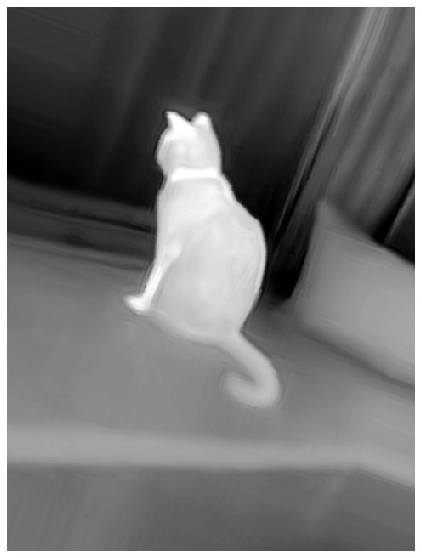
\includegraphics[width=\textwidth]{images/augmentation/rotated.png}
    \caption{Rotated $20^{\circ}$}
  \end{subfigure}
  \begin{subfigure}[h!]{0.24\textwidth}
    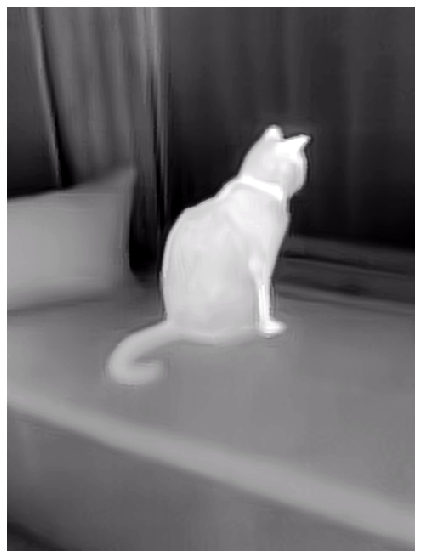
\includegraphics[width=\textwidth]{images/augmentation/flipped.png}
    \caption{Horizontally flipped}
  \end{subfigure}
  \caption{Affine data augmentation strategies applied to a sample LWIR image.}
  \label{fig:augmentation_affine}
\end{figure}

Another possible way of augmenting the data before classification is artificially drawing obstacles over the images. This approach could possibly help the model generalise better on the dataset, as a significant amount of samples from certain classes is obstructed by metal grids or foliage. However, this would require further investigation into the different properties of visible light and LWIR images and their interaction with different types of obstacles. Hence, this approach was not implemented in this project. Instead, we decided to remove a significant part of obstructed samples from the final dataset and focused on working with less noisy data. 

A limitation that remains with all non-generative data augmentation techniques is that the augmented images are not fully independent from each other. The classifier only learns a limited amount of new features from augmented samples. White-box data augmentation can, therefore, only slightly mitigate the problem of insufficient independent samples. To achieve better generalisability, obtaining more data is preferable to augmenting existing data.

%----------------------------------------------------------------------------------------------------------------------------------

\section{Image registration}
\label{image_registration}

As a result of the misalignment of LWIR and VIS images outlined in Section \ref{sensory_equipment}, an algorithm for aligning the images captured by the conventional camera and LWIR camera had to be developed. The process of transforming data from different sensors into one coordinate system is commonly referred to as image registration.

To obtain workable reference samples, multiple images of three candles on a table were captured. The flames of the candles are small, bright and hot enough to function as reference points. Figure \ref{fig:linear_trans_before} displays a thresholded combined VIS and LWIR image of the three candle lights. Upon cursory inspection, it is apparent that the LWIR sensor appears to have a narrower field of view than the RGB camera. Hence, an attempt was made to manually align the LWIR and RGB images by cropping and rescaling the RGB image, effectively zooming in. This approach yielded moderate results, as can be seen in Figure \ref{fig:linear_trans_zoom}.

To obtain a more flexible and generalisable representation, we made use of affine transformations. As shown in Equation \ref{eqn:affine}, an affine transformation can be expressed as a linear function with parameters $A$ and $\vec{b}$. These parameters can be easily trained using a linear regression model. Therefore, the coordinates of about a dozen reference points were manually determined on the RGB and LWIR versions of some test images. These respective coordinates were used as features and labels for training the linear regression model. 

\begin{figure}[ht]
  \centering
  \begin{subfigure}[h!]{0.3\textwidth}
    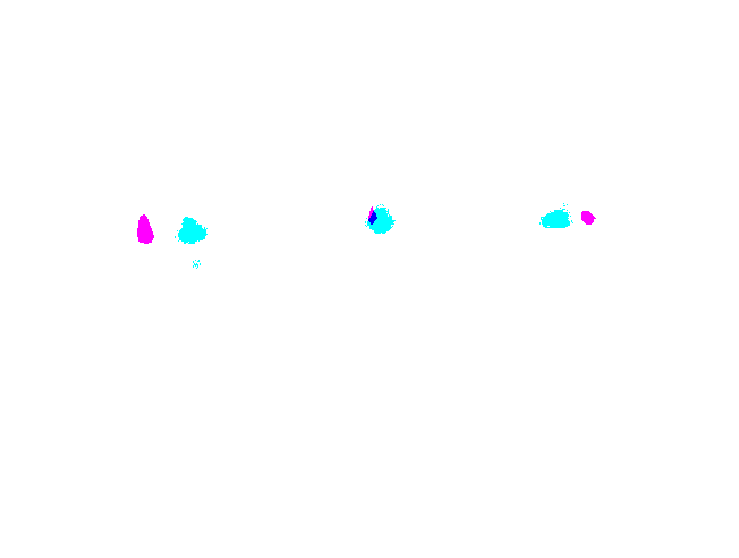
\includegraphics[width=\textwidth, trim={3.5cm 9cm 3.5cm 4.5cm}, clip, frame={\fboxrule} {-\fboxrule}]{images/registration/unregistered.png}
    \caption{Before registration. The LWIR and VIS images are visibly misaligned.}
    \label{fig:linear_trans_before}
  \end{subfigure}
  \quad
  \begin{subfigure}[h!]{0.3\textwidth}
    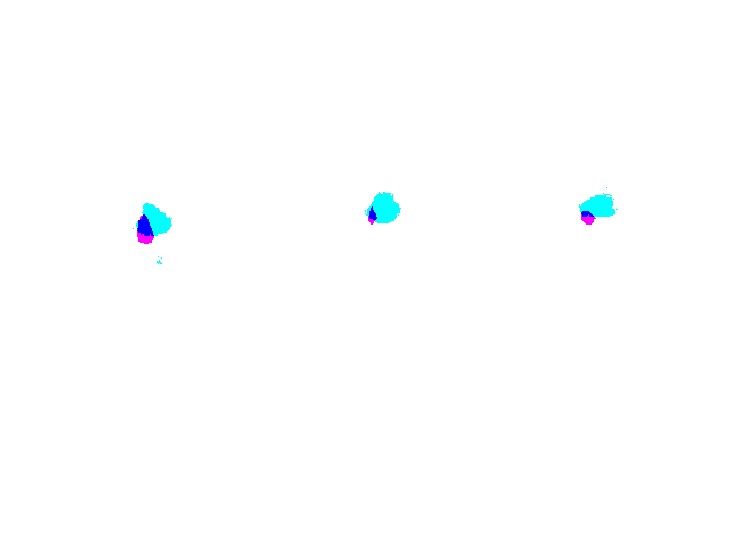
\includegraphics[width=\textwidth, trim={3.5cm 9cm 3.5cm 4.5cm}, clip, frame={\fboxrule} {-\fboxrule}]{images/registration/registered_zoom.png}
    \caption{After zooming in. The images are almost aligned. A slight offset remains.}
    \label{fig:linear_trans_zoom}
  \end{subfigure}
  \quad
  \begin{subfigure}[h!]{0.3\textwidth}
    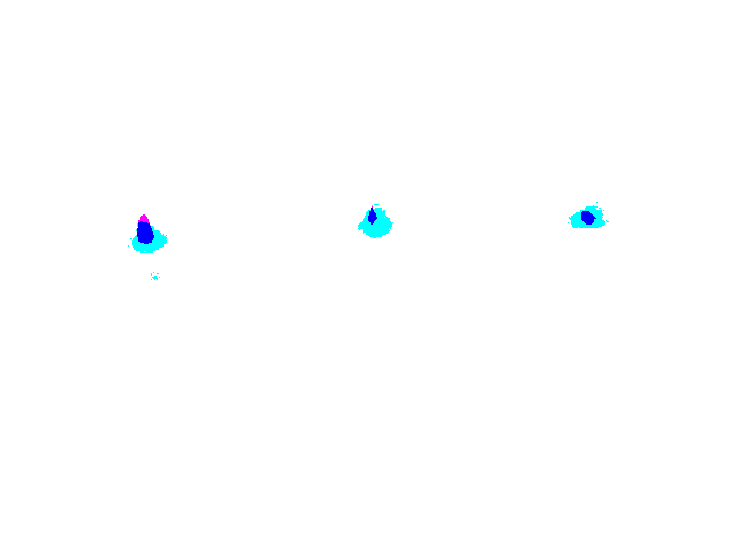
\includegraphics[width=\textwidth, trim={3.5cm 9cm 3.5cm 4.5cm}, clip, frame={\fboxrule} {-\fboxrule}={\fboxrule}]{images/registration/registered_affine.png}
    \caption{After registration. The thermal signatures of the candles align with the VIS location.}
    \label{fig:linear_trans_affine}
  \end{subfigure}
  \caption{Superimposed thresholded LWIR and VIS images before and after registration. Cyan represents the grayscale version of the VIS image and the magenta represents the LWIR image.}
\end{figure}

This approach yielded acceptable results. As can be seen in Figure \ref{fig:linear_trans_affine}, the candles in the images line up. However, manually defining reference points is a time-consuming task, and the quality of alignment is dependent on the precision of those points. To quantify the accuracy of the alignment, attempts were made to use various metrics for image similarity. Such metrics could be used as loss functions for a machine learning model for automatically aligning the channels.

This task is difficult due to the modality gap between VIS and LWIR images. A simple intensity-based metric is unlikely to be successful in this scenario, as local intensities will vary across different channels even if the registration is perfect \citep{myronenko_intensity-based_2010}.

\subsection{Intensity-based registration metrics}

To mitigate the problem of varying intensities across different channels, \citet{chen_normalized_2018} introduce the normalized total gradient (NTG) metric for multispectral imaging systems, which is defined as follows:

\begin{equation}
  NTG(f, f_R) = \frac{\sum_l |\nabla_l \{f - f_R\}|}{\sum_l | \nabla_l f | + \sum_l | \nabla_l f_R|},
\end{equation}

where $f$ and $f_R$ are the channel images to be compared, $\nabla_l$ represents the gradient computation along the direction $l \in \{x, y\}$, and $| \cdot |$ denotes the L1-norm. In other words, to obtain NTG one computes the sum of the $x$- and $y$-gradients of the difference of the two channels, and normalises the result by dividing over the sum of gradients of the individual channels.

The metric is based on the assumption that the gradient of the channel difference image becomes sparser as the alignment improves. Figure \ref{fig:gradient_distribution} shows that this is hardly the case for images captured by the LWIR camera, as opposed to the baseline of comparing the red and green channels from the VIS camera.

\begin{figure}[ht]
  \centering
  \begin{subfigure}[h!]{0.45\textwidth}
    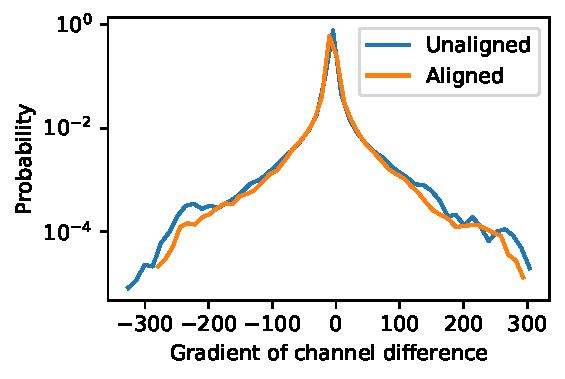
\includegraphics[width=\textwidth]{images/registration/gradient_distribution}
    \caption{LAB intensity of VIS image vs LWIR intensity.}
    \label{fig:gradient_distribution}
  \end{subfigure}
  \begin{subfigure}[h!]{0.45\textwidth}
    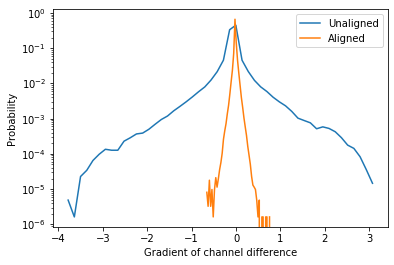
\includegraphics[width=\textwidth]{images/registration/gradient_distribution_red_green}
    \caption{Red channel intensity vs green channel intensity.}
    \label{fig:gradient_distribution_red_green}
  \end{subfigure}
  \caption{Distribution of gradients of the channel difference image before and after alignment using affine transformation. While the gradient distribution of the red and green channel difference gets sparser upon alignment \subref{fig:gradient_distribution_red_green}, it remains mostly unchanged for the VIS and LWIR channels \subref{fig:gradient_distribution}.}
\end{figure}

An attempt at smoothing both images before calculating the NTG was made by applying the Laplacian of Gaussian (LoG) filter with $\sigma=2$ to both images. As can be seen in Table \ref{table:registration_ntg}, this approach was not successful either. To verify that our implementation of the metric was indeed working correctly, we computed the NTG between the red and green channel of the visible-light image before and after applying a random affine transformation to the green channel. As shown in Table \ref{table:registration_ntg}, the metric is effective for the red-green-channel baseline. 

\begin{table}[ht]
  \centering
  \begin{tabular}{@{}lll@{}}
    \toprule
    \textbf{Test configuration}                               & \textbf{Misaligned} & \textbf{Aligned} \\ \midrule
    LAB intensity of VIS vs LWIR                              & 0.9974              & 0.9986           \\
    LAB intensity of VIS (after LoG with $\sigma=2$) vs LWIR  & 0.9970              & 0.9973           \\
    (Baseline) Red vs green channels of VIS                   & 0.6245              & 0.0303           \\ \bottomrule
  \end{tabular}
  \caption{Normalized Total Gradient before and after manual registration of the channels.}
  \label{table:registration_ntg}
\end{table}

Considering these results, we concluded that NTG does not appear to be a suitable metric for this particular registration problem. Since the algorithm is effective on the baseline, it is likely that the modality gap between the LWIR and RGB channels is too significant for an intensity-based approach.

\subsection{Texture-based registration}

Having demonstrated that state-of-the-art intensity-based metrics appear to be inadequate to quantify the registration of visible-light and LWIR images, an approach based on image texture features, as proposed by \citet{jarc_graz_2007} was tested. 

The method uses pairs of 1-D filter masks as introduced by \citet{laws_rapid_1980} to detect level, edge, spot and ripple features. These filters can be applied horizontally and vertically. In our implementation, all possible filter pairs were evaluated. After convoluting both the LWIR and RGB images with the filters, the results were turned into texture energy images by performing a convolutional sum-operation of absolute values using a $15 \times 15$ kernel and applying a threshold of $\pm 3 \sigma$. Figure \ref{fig:le_filter} shows corresponding VIS and LWIR images after applying the \textit{level} kernel horizontally and the \textit{edge} kernel vertically.

\begin{figure}[ht]
  \centering
  \begin{subfigure}[h!]{0.25\textwidth}
    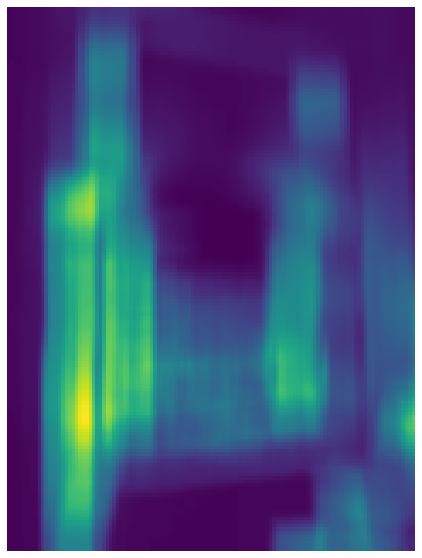
\includegraphics[width=\textwidth]{images/registration/filtered_le_rgb.png}
    \caption{VIS}
  \end{subfigure}
  \begin{subfigure}[h!]{0.25\textwidth}
    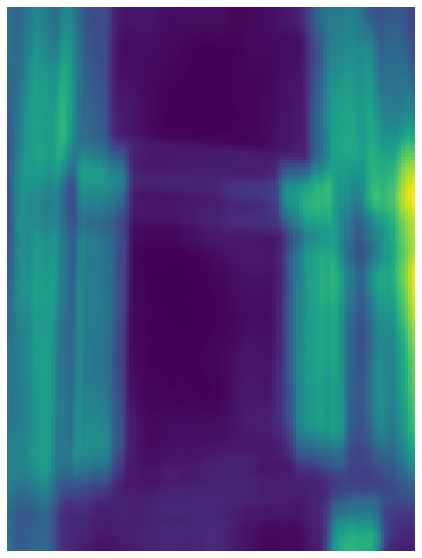
\includegraphics[width=\textwidth]{images/registration/filtered_le_lwir.png}
    \caption{LWIR}
  \end{subfigure}
  \caption{Effect of LE-Kernel \citep{laws_rapid_1980} on visible-light and LWIR images.}
  \label{fig:le_filter}
\end{figure}

Finally, the mutual information (MI) of the resulting LWIR and VIS texture energy images was calculated as follows:

\begin{equation}
  MI(A,B) = H(A) + H(B) - H(A,B),
\end{equation}

where $H(X) = - \sum_{x \in X} p(x) \cdot \log_2 p(x)$ is the entropy of $X$ and $H(X,Y)$ represents the joint entropy of $X$ and $Y$.

We then averaged the MI scores obtained by all 1-D filter pairs to calculate a single metric. For the test samples, the MI score did not appear to change consistently when aligning the images. Furthermore, none of the individual MI values for the different filter combinations behaved reliably across all samples. Hence, we deemed this approach ineffective for our registration problem.

\subsection{Mean distance}
\label{mean_distance}

Since neither intensity-based nor texture-based approaches produced satisfactory results, we concluded that an automatic registration of the visible-light and LWIR images was unfeasible without extensive further research. Therefore, to be able to guarantee an acceptable alignment quality across the whole dataset, we resorted back to manual alignment.

For this purpose, 97 reference points were manually determined from the training data. One image was drawn from each of the 35 subsets, ensuring that all available camera orientations and perspectives were incorporated into the model. The coordinates were rescaled to $120 \times 160$, which is the desired input resolution for the CNNs. Subsequently, by fitting a linear regression model, the transformation parameters were determined to be: 

\begin{equation}
  A = \begin{pmatrix}
    1.260 & -0.016  \\
    0.020 & 1.192
  \end{pmatrix}, \ 
  \vec{b} = \begin{pmatrix}
    -14.619  \\
    -18.660
  \end{pmatrix}.
  \label{trans}
\end{equation}

Prior experiments showed that the required transformation seems to be mostly consistent across different images. Device orientation appears to be the only factor with a large impact on the required transformation. To avoid this problem, all images were captured in portrait mode. Figure \ref{fig:registration_relationship} shows the relationship between the re-scaled visible-light and LWIR coordinates across both dimensions. The relationship appears to be linear. However, it can be seen that the gradient for the relationship of horizontal coordinates is slightly steeper than for the vertical coordinates. This supports the necessity to perform an affine transformation, as opposed to just zooming in.

\begin{figure}[ht]
  \centering
  \begin{subfigure}[t]{0.45\textwidth}
    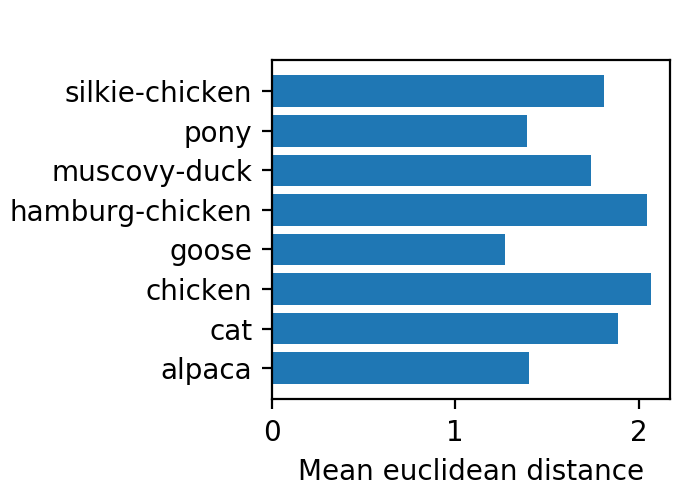
\includegraphics[width=\textwidth]{images/registration/error}
    \caption{Mean distance between predicted and actual LWIR coordinates.}
    \label{fig:registration_error}
  \end{subfigure}
  \quad
  \begin{subfigure}[t]{0.368\textwidth}
    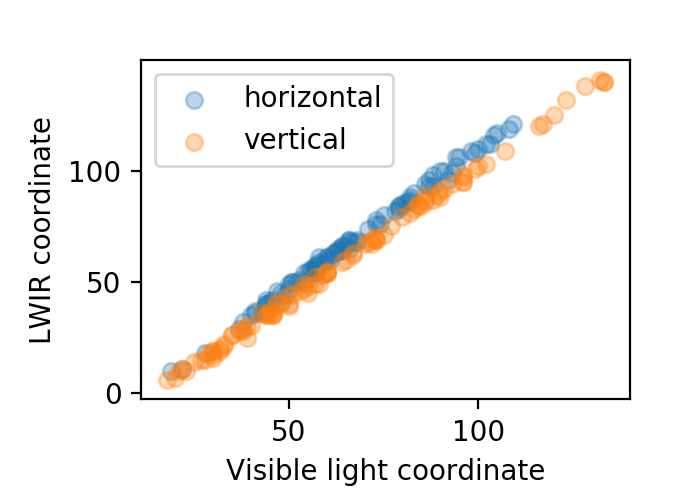
\includegraphics[width=\textwidth]{images/registration/x_y}
    \caption{Relationship between reference points in VIS and LWIR images.}
    \label{fig:registration_relationship}
  \end{subfigure}
  \caption{Results of manual registration of LWIR and VIS images.}
\end{figure}

To quantitatively evaluate whether the transformation parameters generalise across all images, the mean euclidean distance between the actual LWIR coordinates and the ones predicted by the regression model was computed for every class in the dataset. The results can be seen in Figure \ref{fig:registration_error}. The highest mean distance is around 2, which we consider small considering the image resolution. These errors are likely due to noise in the manually determined reference points. The mean distance across all reference points in the dataset was determined to be around 1.777 with $\sigma = 0.589$.

When using convolutional kernels with a small size, such as $3 \times 3$, this distance could, however, be problematic, as edges and other features might not be picked up consistently across channels.

%----------------------------------------------------------------------------------------------------------------------------------

\section{Classifiers}
\label{design_classifiers}

Following the conclusion of \citet{wagner_multispectral_2016} about the effectiveness of early and late fusion techniques, we decided to implement and evaluate early fusion, late fusion and score-level-based fusion classifiers. These three multispectral neural network architectures are shown in Figure \ref{fig:archs}.

\begin{figure}[ht]
  \centering
  \begin{subfigure}[h!]{0.3\textwidth}
    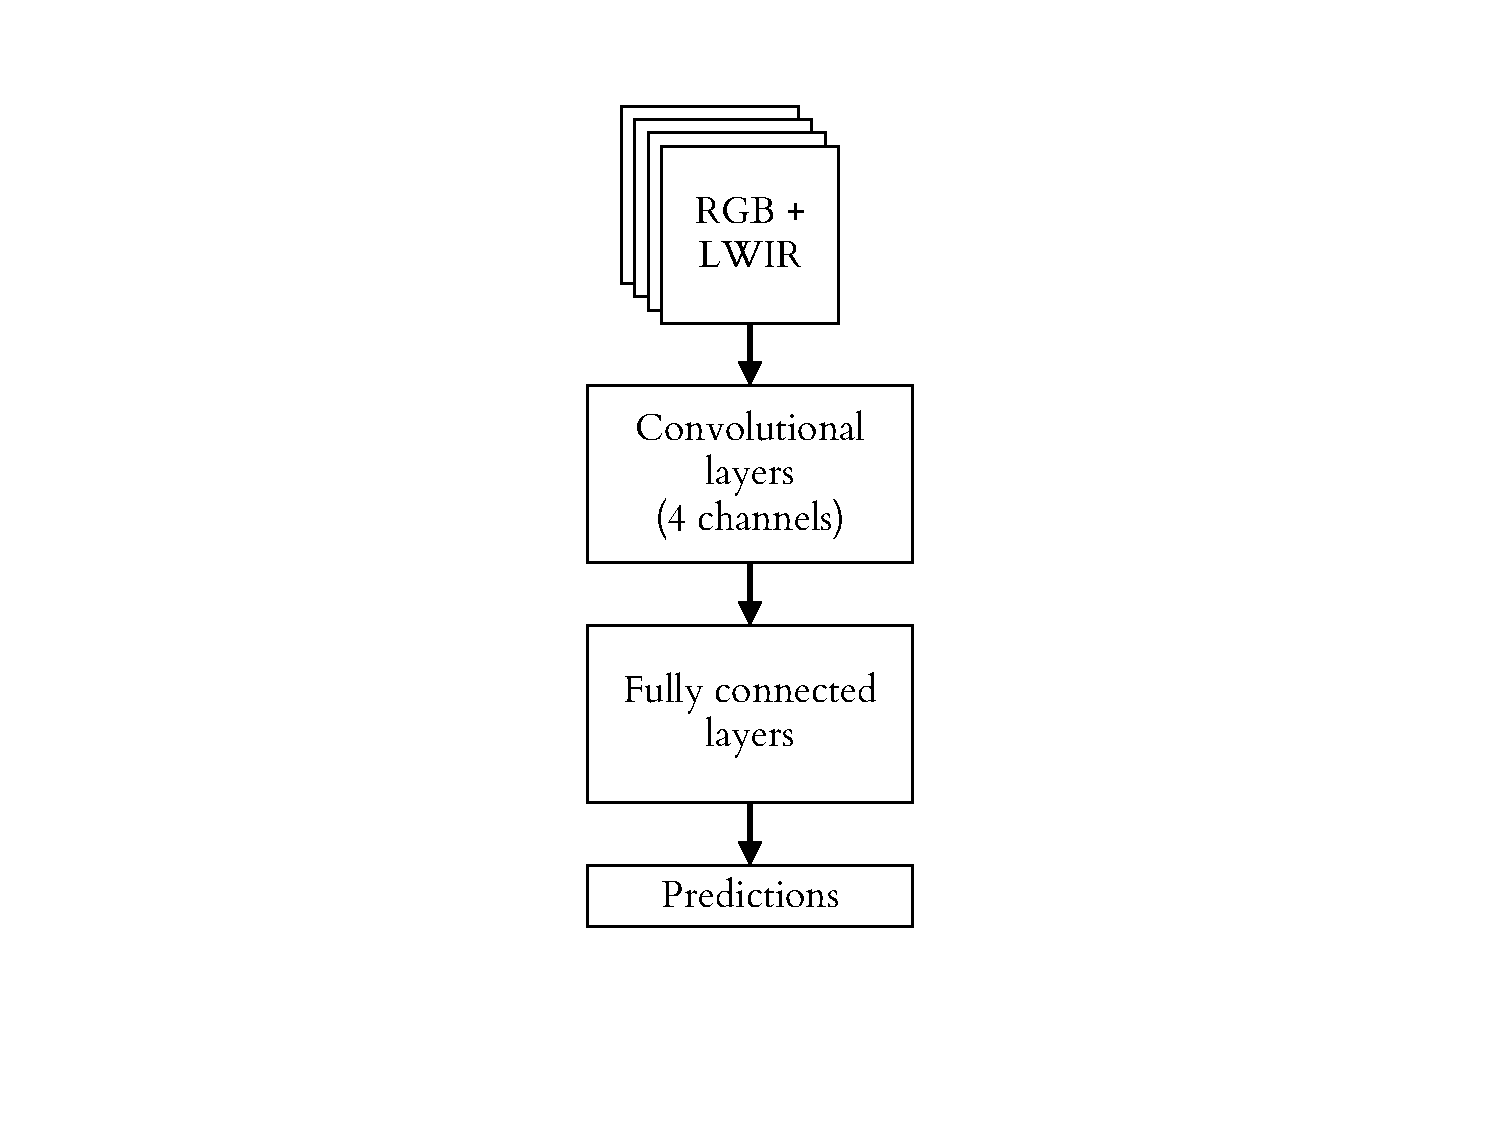
\includegraphics[width=\textwidth, page={1}, trim={6.5cm 2.2cm 6.5cm 1.5cm}, clip]{images/models/archs}
    \caption{Pixel-based early fusion.}
    \label{fig:arch_stacked}
  \end{subfigure}
  \quad
  \begin{subfigure}[h!]{0.3\textwidth}
    \includegraphics[width=\textwidth, page={2}, trim={6.5cm 2.2cm 6.5cm 1.5cm}, clip]{images/models/archs}
    \caption{Score-based fusion.}
    \label{fig:arch_combsum}
  \end{subfigure}
  \quad
  \begin{subfigure}[h!]{0.3\textwidth}
    \includegraphics[width=\textwidth, page={3}, trim={6.5cm 2.2cm 6.5cm 1.5cm}, clip]{images/models/archs}
    \caption{Late fusion.}
    \label{fig:arch_fusion}
  \end{subfigure}
  \caption{Multispectral CNN configurations that were implemented for each CNN architecture.}
  \label{fig:archs}
\end{figure}

In total, we implemented five configurations of each of the CNN designs outlined in the Sections \ref{custom_cnn}, \ref{alexnet} and \ref{resnet}:

\begin{enumerate}
  \item An RGB-only configuration, similar to the default implementation of most networks. This configuration provides a baseline for our multispectral models, as it resembles the capabilities of conventional VIS-only computer vision.
  \item An LWIR-only implementation. This configuration allows us to compare the isolated performance of LWIR-based and VIS-based classifiers for our dataset.
  \item A pixel-based early fusion implementation. The RGB and LWIR channels are stacked into a tensor of shape $({batch\ size} \times width \times height \times 4)$. This tensor is then fed into the network. This configuration is shown in Figure \ref{fig:arch_stacked} and is referred to in evaluation figure legends as \textit{stacked} mode.
  \item A score-level fusion implementation with soft-voting classifiers. The VIS and LWIR images are run through separate CNNs, producing separate predictions. The final output of the classifier is the mean of these two predictions. This configuration can be seen in Figure \ref{fig:arch_combsum} and is labelled \textit{voting} mode in figure legends.
  \item A multi-branch implementation with late feature-level fusion, as shown in Figure \ref{fig:arch_fusion}. Here, the RGB and LWIR images are fed into separate branches of convolutional layers. The respective outputs are flattened, concatenated and fed into the fully-connected layers at the end of the network, producing the final prediction. This configuration is referred to as \textit{fusion} mode in figure legends.
\end{enumerate}

Furthermore, three different CNN designs were evaluated. At first, a custom neural network was designed and implemented. In addition, we implemented modified versions of AlexNet and ResNet, two CNNs commonly used for image classification tasks. 

Note that the following architecture diagrams (Figures \ref{fig:customnet}, \ref{fig:alexnet} and \ref{fig:resnet}) show the RGB-only configurations of the networks. The other configurations can be derived from these and the architectural visualisation in Figure \ref{fig:archs}. To provide a tangible example, Appendix \ref{appendix_arch} contains the detailed multispectral configurations of our AlexNet implementation.

\subsection{Custom CNN}
\label{custom_cnn}

A custom CNN architecture, as shown in Figure \ref{fig:customnet}, was implemented. The network follows a typical design pattern for image classifiers, chaining multiple convolutional and pooling layers with increasing amounts of filters, followed by a small number of fully-connected layers. Our model consists of two blocks that are each composed of two convolutional layers, a ReLU activation function, and a max-pooling layer. Following the convolutional blocks, we added a fully-connected (FC) layer and an output layer with softmax activation. Dropout regularisation is applied to the outputs of the FC layer to reduce overfitting.

\begin{figure}[ht]
  \centering
  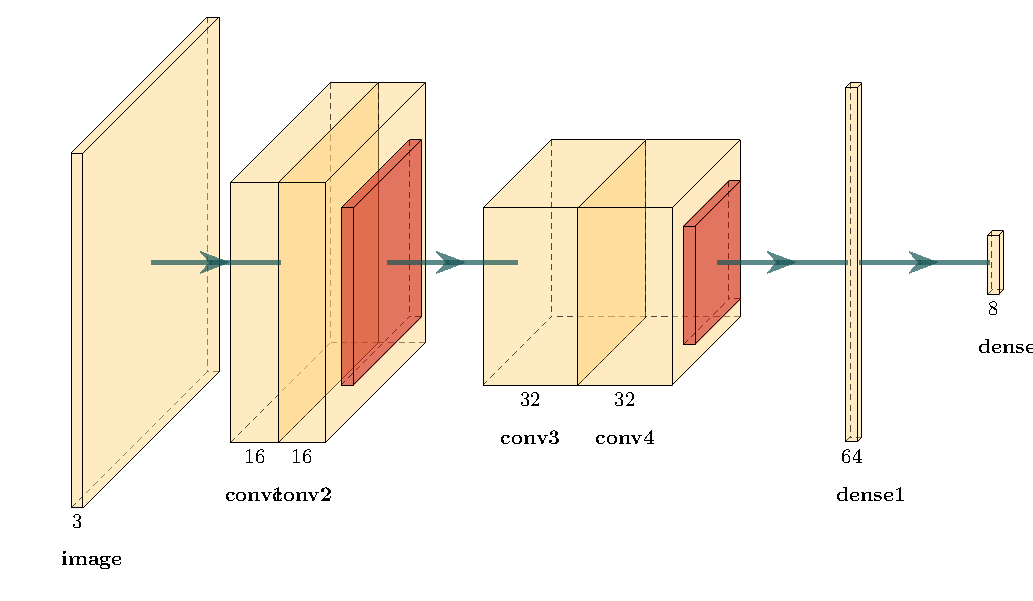
\includegraphics[width=0.65\textwidth]{images/models/customnet}
  \caption{Architecture of the custom CNN. Created using PlotNeuralNet \citep{iqbal_harisiqbal88plotneuralnet_2018}.}
  \label{fig:customnet}
\end{figure}

Pooling operations are an unsupervised non-linear method for downsampling inputs. Max-pooling works by dividing the input map into discrete, non-overlapping regions and outputting the maximum value of each region. The result is a feature map of reduced size. Pooling layers are commonly used in CNNs to achieve positional invariance and extract dominant features from the output of convolutional layers. \citet{scherer_evaluation_2010} state max-pooling as a superior method for capturing invariant features in image data compared to alternative strategies.

Overall, the model has $117\,592$ trainable weights. This architecture was designed as a low-end model with relatively few parameters that is fast to train and evaluate.

\subsection{AlexNet}
\label{alexnet}

AlexNet was first introduced by \citet{krizhevsky_imagenet_2012}, winning the ImageNet Large Scale Visual Recognition Challenge (ILSVRC). Significantly outperforming the state-of-the-art traditional image classification models of its time, AlexNet is considered a significant breakthrough in computer vision \citep{alom_history_2018}.

The architecture of AlexNet consists of an initial convolutional layer with a relatively large kernel size of $11 \times 11$, feeding into a max pooling layer. This is followed by a second block of convolutional and pooling layers. The kernel size of the second convolutional layer is $5 \times 5$. Subsequently, three convolutional layers with $3 \times 3$ kernels are applied, followed by another pooling layer. Finally, the output is fed into two subsequent fully connected layers, followed by an output layer with a softmax activation function.

We decided to evaluate an implementation of AlexNet due to various factors. Firstly, the model has delivered good results on many image classification tasks. Simultaneously, its architecture can be considered shallow compared to most modern-day networks. This makes it likely that AlexNet will be able to run with low latency on a mobile edge device. Finally, the first convolutional layer of AlexNet has a large kernel compared to most modern-day networks. This might help mitigate the misalignment problem discussed in Section \ref{mean_distance}.

\begin{figure}[ht]
  \centering
  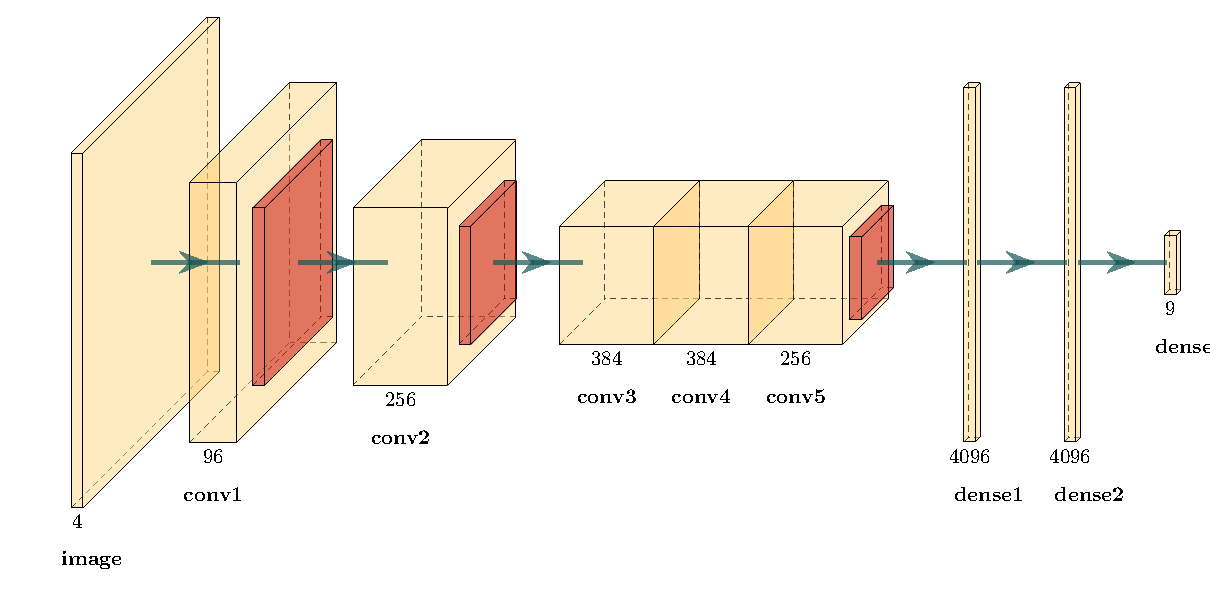
\includegraphics[width=0.9\textwidth]{images/models/alexnet}
  \caption{Neural network architecture of AlexNet. Created using PlotNeuralNet \citep{iqbal_harisiqbal88plotneuralnet_2018}.}
  \label{fig:alexnet}
\end{figure}

Our implementation of AlexNet, as shown in Figure \ref{fig:alexnet} diverges slightly from the original. Due to a lower input resolution and a smaller number of resulting parameters, the FC layers at the end of the network only have 1024 instead of 4096 parameters each. Furthermore, we included dropout layers after both FC layers to combat overfitting. In total, our AlexNet implementation has $7\,951\,752$ trainable parameters in the RGB-only configuration.

\subsection{ResNet}
\label{resnet}

Since the initial introduction of AlexNet, many more CNN-architectures have been developed. \citet{simonyan_very_2015} proposed VGG, a neural network with a substantially increased number of convolutional layers. VGG demonstrates that deeper networks are more likely to perform well on image classification tasks than shallow architectures \citep{alom_history_2018}.

ResNet was developed by \citet{he_deep_2016}. Winning the 2015 ILSVRC, ResNet is considered a state-of-the-art neural network for image classification. It makes heavy use of a novel design component known as a residual block. 

\begin{figure}[ht]
  \centering
  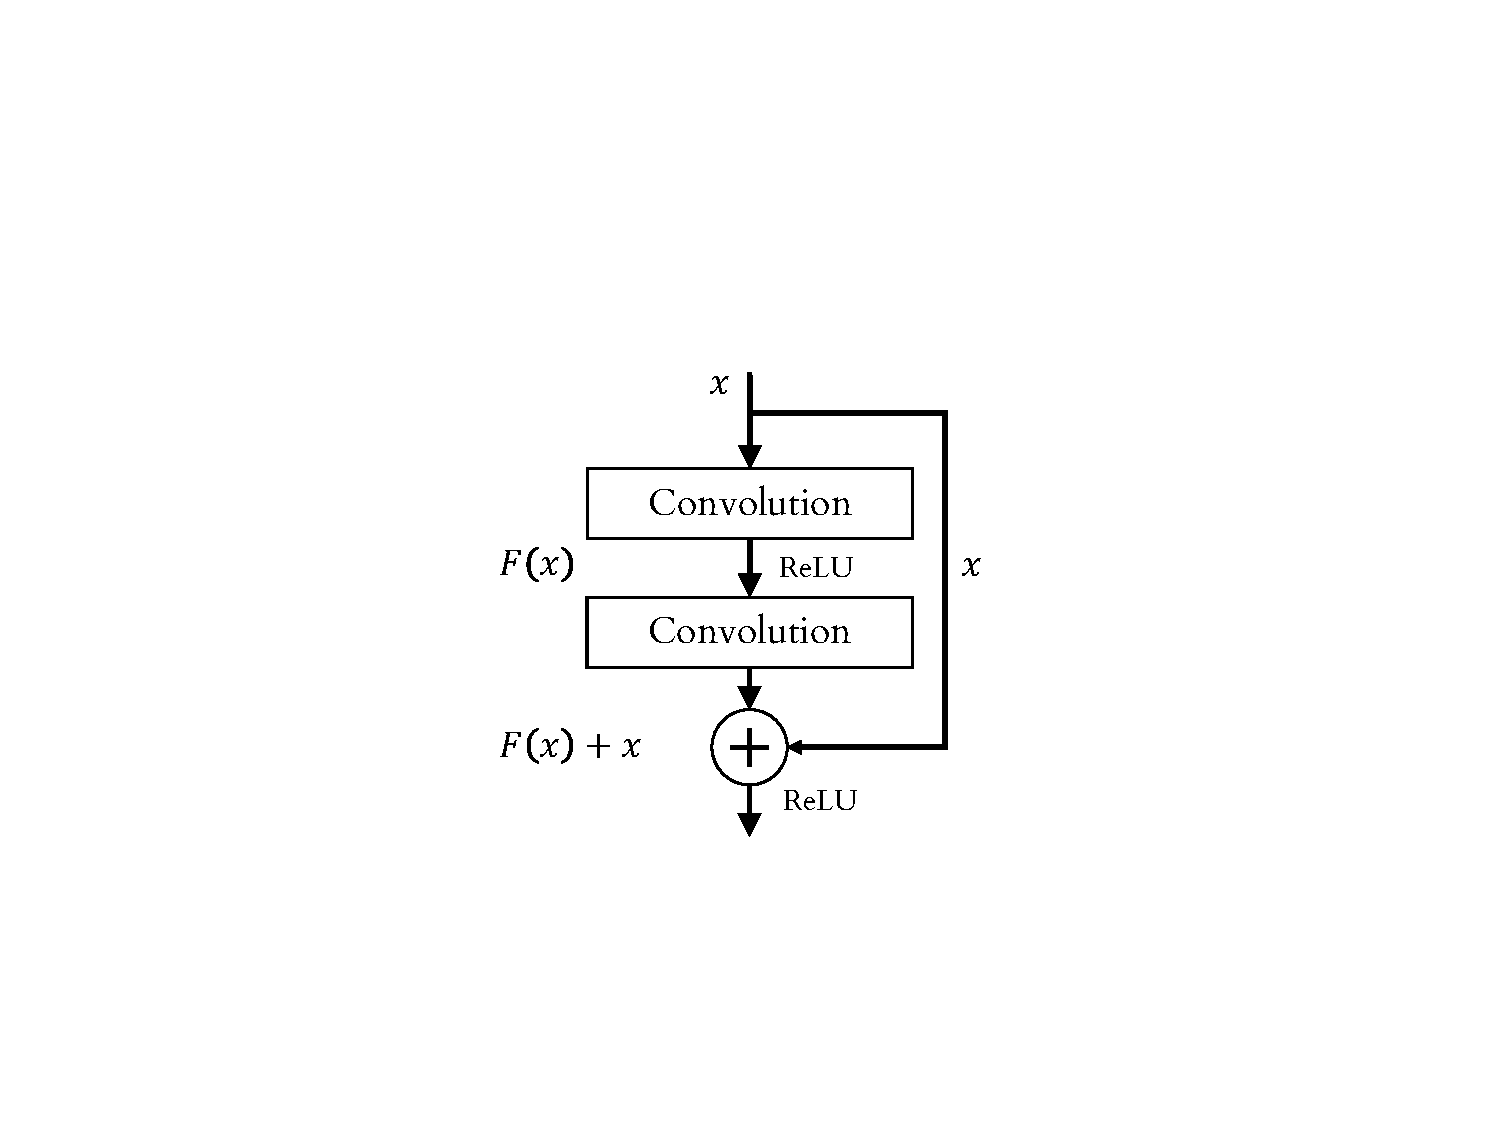
\includegraphics[width=0.45\textwidth, trim={7cm 4.8cm 7cm 6cm}, clip]{images/models/res_block}
  \caption{Schematic of a residual block with 2 convolutional layers.}
  \label{fig:res_block}
\end{figure}

Figure \ref{fig:res_block} shows an example residual block. The input to the block is fed into multiple subsequent convolutional layers with ReLU activation functions. The outputs of the last convolutional layer $F(x)$ are then added to the identity of the initial input $x$. This architecture allows the propagation of earlier features into later layers and helps avoid the problem of vanishing gradients that most predecessor architectures encountered \citep{alom_history_2018}. As a result, significantly deeper network designs can be created, most likely outperforming existing shallower architectures.

\begin{figure}[ht]
  \centering
  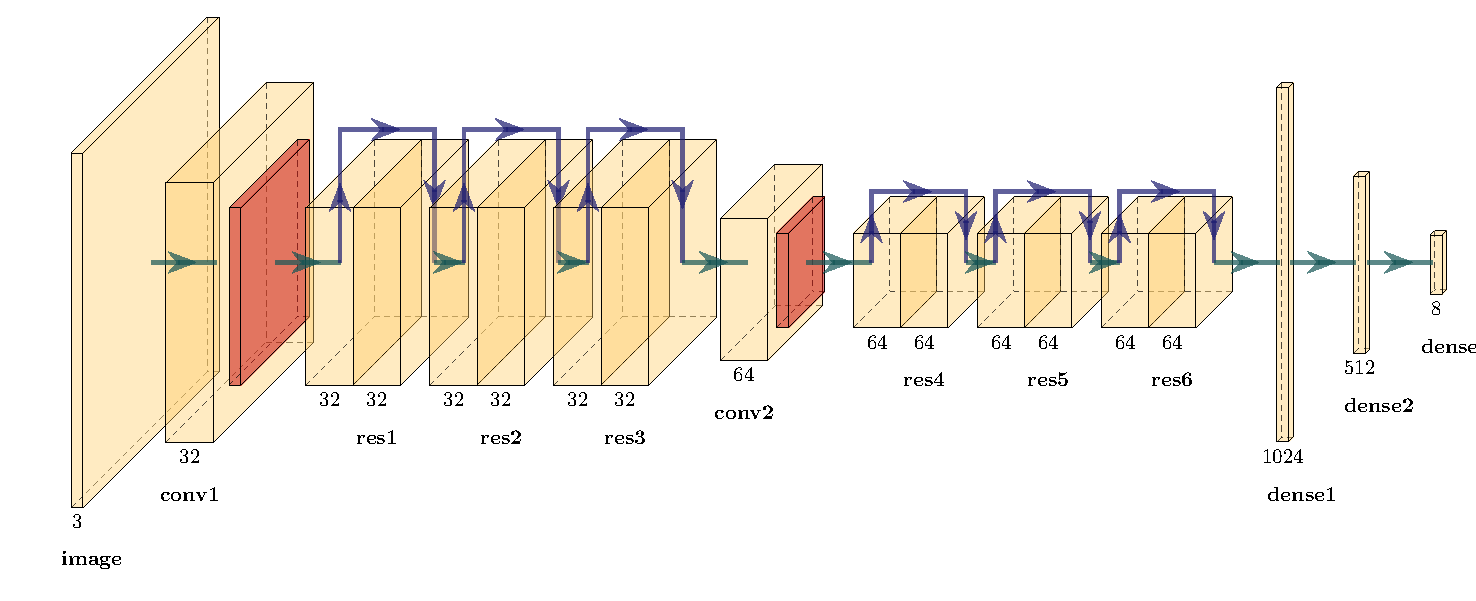
\includegraphics[width=0.9\textwidth]{images/models/resnet}
  \caption{Neural network architecture of the residual network. Created using PlotNeuralNet \citep{iqbal_harisiqbal88plotneuralnet_2018}.}
  \label{fig:resnet}
\end{figure}

The original paper proposes implementations of ResNet with 50, 101 and 152 layers. Since our dataset is significantly smaller than ImageNet, it is likely that these models would overfit on the training data without adding much benefit over a shallower architecture. Hence, we decided to implement a custom version of ResNet with six residual blocks and a total of 14 convolutional layers. The architecture can be seen in Figure \ref{fig:resnet}.

The residual blocks are arranged in two groups of three. The convolutional kernels of each block have size $5 \times 5$. Each group of residual blocks is preceded by a single convolutional layer with a max pooling layer to reduce the input resolution. Unlike in the original paper, we use two FC layers with dropout in the end, followed by a softmax-activated output layer. Despite the much deeper architecture compared to AlexNet, our ResNet implementation has only $4\,033\,160$ trainable parameters.

%----------------------------------------------------------------------------------------------------------------------------------


\section{Transfer learning using a pre-trained ResNet}
\label{transfer_learning}

An attempt was made to make use of transfer learning. We decided to evaluate an RGB-only, LWIR-only and late fusion configuration of a pre-trained network. 

Obtaining an RGB-only network with pre-trained weights is easy. We used an implementation of ResNet 152 v2 \citep{he_identity_2016} with weights that were previously trained on the ImageNet dataset. Since ImageNet has 1000 classes, we had to replace the output layer of the network with a custom layer, to make labels and outputs match.

As discussed in Section \ref{transfer_learning_analysis}, limited resources are available for transfer learning of thermal images. After some review, an annotated thermal dataset provided by FLIR was found \footnote{\url{https://www.flir.com/oem/adas/adas-dataset-form/}}. This dataset was deemed suitable because it was captured by another FLIR camera, minimising the sensor difference. Nonetheless, at $640 \times 512$, the thermal infrared resolution of the FLIR Tau 2 is significantly higher than that of the FLIR One Pro ($160 \times 120$) used for this project. The dataset contains a total of $10\,228$ frames with bounding box annotations for five classes: \textit{person}, \textit{car}, \textit{bicycle}, \textit{dog} and \textit{other vehicle}.

To use the bounding box annotations for our classification problem, we treated each bounding box as an individual sample, cropping the images appropriately. To reduce noise, we removed samples with a resolution below $40 \times 40$. Only thermal images were used. We then trained an off-the-shelf implementation of ResNet 50 v2 on this dataset. We chose this shallower version of ResNet due to the limited amount of available data and time. It was deemed unlikely that using a more complex, such as ResNet 152 v2 model would benefit performance significantly.

The late fusion configuration of our transfer learning model, therefore, uses a ResNet 152 v2 for the RGB path, and a ResNet 52 v2 for the LWIR path.

%----------------------------------------------------------------------------------------------------------------------------------

\section{Mobile application design}

The mobile application was designed with two primary user requirements in mind:

\begin{enumerate}
  \item Giving users the ability to capture combined visible-light and thermal datasets. For this purpose, easy access to the captured raw images shall be provided.
  \item Being able to perform real-time multi-class classification using the CNNs designed in Section \ref{design_classifiers}.
\end{enumerate}

Following the analysis in Section \ref{analysis_mobile_application}, we decided to perform all necessary computations on-device. This means that the application does not require an active internet connection to perform real-time classification. 

The application comprises of a camera activity and a classifier activity that are each designed to meet one of the two requirements. Both activities display the live image feed from the FLIR camera. The camera view, furthermore, has a button to start and stop the capture mode. When enabled, each frame captured by the FLIR camera is saved to device storage and added to the gallery.

The classifier activity shows the top three predictions of the current image at the top of the screen. Both activities contain a toggle switch to enable and disable image registration. When activated, the affine transformation from Equation \ref{trans} is applied to the VIS images from the FLIR camera, before displaying them or feeding them into the classifier.

%==================================================================================================================================
\chapter{Implementation}
\label{implementation}

\section{Frameworks and tools}

\subsection{Mobile application development}

The mobile application was developed using Android Studio and the Java programming language. To communicate with the FLIR sensor, we used the FLIR Thermal SDK for Android. A continuous delivery (CD) build pipeline was set up using GitHub Actions to verify that changes to the application do not include build-breaking bugs. To achieve this, the pipeline automatically downloads software dependencies, such as the FLIR SDK, compiles the application and provides a downloadable and installable APK file.

\subsection{Deep learning and image processing}

All neural networks were implemented using the TensorFlow deep learning framework \citep{abadi_TensorFlow_2016}. TensorFlow was chosen over alternatives such as PyTorch due to its built-in Keras API and its compatibility with TensorFlow Lite. Keras is a high-level neural networks API that was developed by \citet{chollet_keras_2015} to enable fast experimentation. Keras was used in conjunction with other modules provided by the TensorFlow library. 

TensorFlow Lite is a set of tools aimed towards running deep learning models on mobile and internet of things (IoT) devices. It provides a Java API that can be used for Android application development and was, therefore, selected for the deployment of the model onto a mobile device.

To perform the various image processing tasks required for this project, we made use of scikit-image \citep{van_der_walt_scikit-image_2014} and the Python implementation of OpenCV \citep{bradski_opencv_2000}. Furthermore, the Java implementation of OpenCV was used for the Android application, making it possible to perform affine transformations on captured images on the edge device.

We computed the Grad-CAM visualisations of our networks using Keras-vis \citep{kotikalapudi_keras-vis_2017}.

\subsection{Hardware and environment}

Training a deep neural network is a time-consuming process. However, many of the operations that get executed when fitting and evaluating a deep learning model benefit from hardware-accelerated vectorised computation. Therefore, training and evaluation of a neural network can be several orders of magnitude faster on a GPU than on a CPU due to the GPU's ability for parallelised computations \citep{shi_benchmarking_2016}. 

Hence, Google Colaboratory (Colab) was used for most of the experimentation process and design of models. Colab is a cloud-hosted service that allows the execution of Jupyter Notebooks on free-to-use GPU runtimes. Therefore, we were able to leverage the power of an Nvidia Tesla P4 GPU with 8 GB of VRAM.

For more computationally expensive tasks, we made use of the GPU cluster provided by the faculty's Information, Data \& Analysis research section. The cluster provides access to nodes with more powerful resources than Colab, including 512 GB of RAM and multiple Nvidia GeForce RTX 2080 Ti GPUs with 24 GB of VRAM.

The cluster uses Openshift and the Kubernetes container management framework to assign resources to jobs. To be able to run computations on the cluster, we created a custom Docker image with all our software requirements, including TensorFlow and OpenCV. When scheduling a job, a container instance is created from this image that executes the supplied training script.

%----------------------------------------------------------------------------------------------------------------------------------

\section{Architecture and implementation details}

\subsection{Data loading}

Due to the limited amount of memory that Colab provides, it is impossible to pre-load the entire training dataset into memory for training. Thus, a data loader class was implemented that supported the lazy loading of data batches. When constructing the loader, a batch size can be specified, in addition to whether image samples shall be registered, and the target image resolution. 

Since the data loader extends Keras' \lstinline{Sequence} class, it fully integrates with the \lstinline{Model} training API. When constructed, it loads a list of all samples, containing image paths and class labels. It then enumerates the classes.

When \lstinline{model.fit()} is called with the data loader as the data source, Keras will use the \lstinline{__getitem__()} function of the data loader repeatedly to lazily load batches of images into memory. The data loader will register images if specified and convert them into a tensor of shape $(batch\_size \times height \times width \times 4)$. Finally, it will return a tuple containing the image tensor and the one-hot representation of the numeric class labels.

While this approach was necessary to fit the model on the whole training dataset, we found that it noticeably slowed down training speeds. This is most likely due to slow I/O bottlenecking the loading speed. Instead of having to load the dataset into memory once in the beginning, loading has to be performed for every training epoch. An attempt was made to use TensorFlow's data API instead of OpenCV for loading and pre-processing to load the data directly into VRAM. However, the performance improvement was negligible. Therefore, when running evaluations on the GPU cluster, we resorted to pre-loading all batches into memory, using our data loader class.

\subsection{Grid search}
\label{gridsearch_impl}

To evaluate the performance of the three different models and the five configurations, a grid search was run over all 15 possible combinations. For this purpose, we derived all models from a custom-built superclass \lstinline{AbstractModel}, to ensure that they implement a common API. This enabled us to iterate over all models and all configurations, training and evaluating every combination.

\subsection{Affine data augmentation}
\label{augmentation_impl}

Various tools are available to perform real-time data augmentation as part of the training pipeline. However, to achieve the highest possible level of control, a custom data augmentation function was designed. The function accepts a multiplication factor $n$ and leverages TensorFlow's \lstinline{ImageDataGenerator} to apply random affine transformations to images in the dataset.

The script works by counting the number of samples per class and determining the class with the highest support. Each sample in that class is then augmented $n$ times. Finally, all remaining classes are being augmented until their sample size reaches that of the max class. The aim of this algorithm is to provide an even dataset without class imbalances.


\subsection{Predicting LWIR images using an autoencoder}
\label{autoencoder_implementation}

\subsubsection{Traditional autoencoder}



A deep convolutional autoencoder was created to predict the LWIR signature of objects from the corresponding visible-light image. The architecture of the network is shown in Figure \ref{fig:autoencoder_architecture}. The network consists of an encoder and a decoder that each contain four blocks of layers.

\begin{figure}[ht]
  \centering
  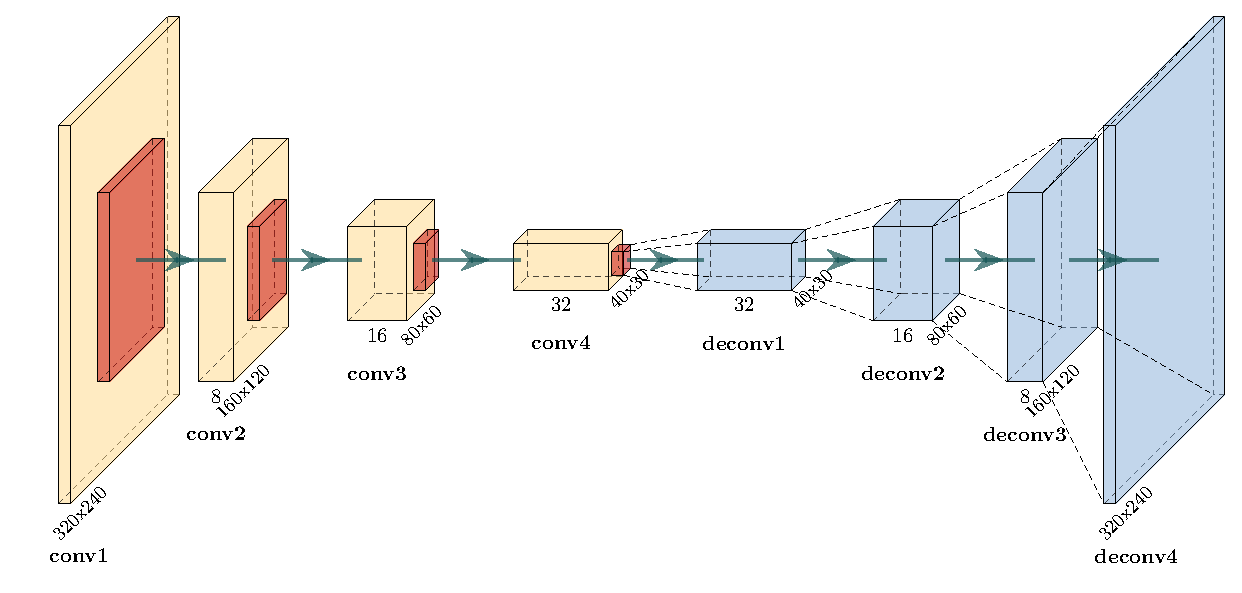
\includegraphics[width=0.9\textwidth]{images/models/autoencoder}
  \caption{Neural network architecture of the autoencoder. Created using PlotNeuralNet \citep{iqbal_harisiqbal88plotneuralnet_2018}.}
  \label{fig:autoencoder_architecture}
\end{figure}

Each encoder block has a convolutional layer, followed by a leaky ReLU activation function and a subsequent max pooling layer for downsampling. The $320 \times 240 \times 1$ input images are thus processed and downsampled to a $20 \times 15 \times 32$ tensor containing a compact, latent representation of the features in the original image.

The output of the decoder is then fed forward into four blocks of deconvolutional layers followed by leaky ReLU activation to attempt a reconstruction of the LWIR image. Each deconvolutional layer tries to upsample the input by predicting appropriate pixel values.

Due to the lack of a discriminator, our autoencoder design does not satisfy the requirements of a generative adversarial network. However, autoencoders are commonly used for image processing tasks such as denoising and colourisation. As LWIR images have fewer high-frequency components than visible-light images (Section \ref{modality}) and both images share rough features such as edges, we deemed an autoencoder architecture to be appropriate for this generative task.

\begin{figure}[ht]
  \centering
  \begin{subfigure}[h!]{0.22\textwidth}
    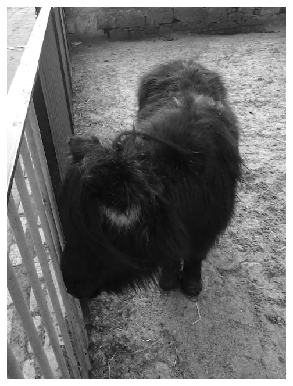
\includegraphics[width=\textwidth]{images/autoencoder/train/gray.png}
    \caption{Original image}
  \end{subfigure}
  \begin{subfigure}[h!]{0.22\textwidth}
    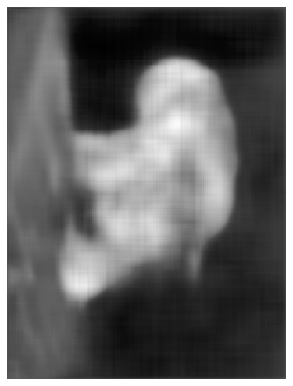
\includegraphics[width=\textwidth]{images/autoencoder/train/auto.png}
    \caption{Autoencoder prediction}
    \label{fig:autoencoder_pony_train_autoencoder}
  \end{subfigure}
  \begin{subfigure}[h!]{0.22\textwidth}
    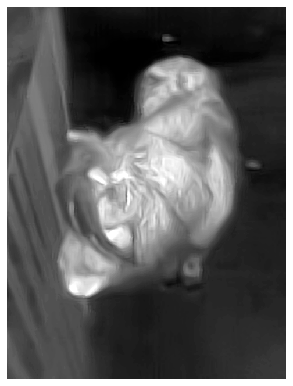
\includegraphics[width=\textwidth]{images/autoencoder/train/unet.png}
    \caption{U-Net prediction}
    \label{fig:autoencoder_pony_train_unet}
  \end{subfigure}
  \begin{subfigure}[h!]{0.22\textwidth}
    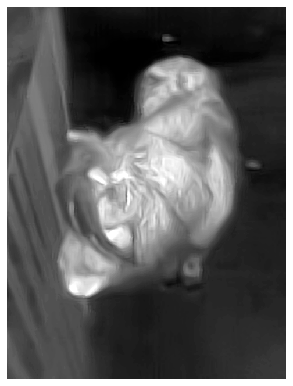
\includegraphics[width=\textwidth]{images/autoencoder/train/lwir.png}
    \caption{Actual LWIR image}
  \end{subfigure}
  \caption{Outputs of autoencoder and U-Net on training data. The U-Net predicts images with more detailed textural information compared to the autoencoder.}
  \label{fig:autoencoder_pony_train}
\end{figure}

A subset of the animals training dataset with 415 images of Shetland ponies was chosen. Mean squared error was selected as the loss function. The network was trained for 100 epochs with a batch size of 16. Training time averaged around 18 minutes on an NVIDIA Tesla P-100 GPU.

As can be seen in Figure \ref{fig:autoencoder_pony_train_autoencoder}, the network correctly identifies the pony from the training dataset and determines that it should have a higher local intensity in the LWIR waveband. However, when comparing the predicted to the actual LWIR image, it is apparent that the autoencoder lacks the ability to generate the fine textural details of the animal. This is likely due to the denoising property caused by the encoder's bottleneck.

\subsubsection{U-Net}

U-Net was first introduced by \citet{ronneberger_u-net_2015} to improve performance of biomedical image segmentation systems. Similarly to a conventional autoencoder, it features a contracting path that downsamples or encodes the input and a symmetric expanding path that upsamples or decodes the input. Additionally, for each deconvolutional layer, the output of the corresponding opposite convolutional layer is concatenated to the layer's input map. These connections can be seen in Figure \ref{fig:unet_architecture}, which visualises our custom U-Net implementation. 

\begin{figure}[ht]
  \centering
  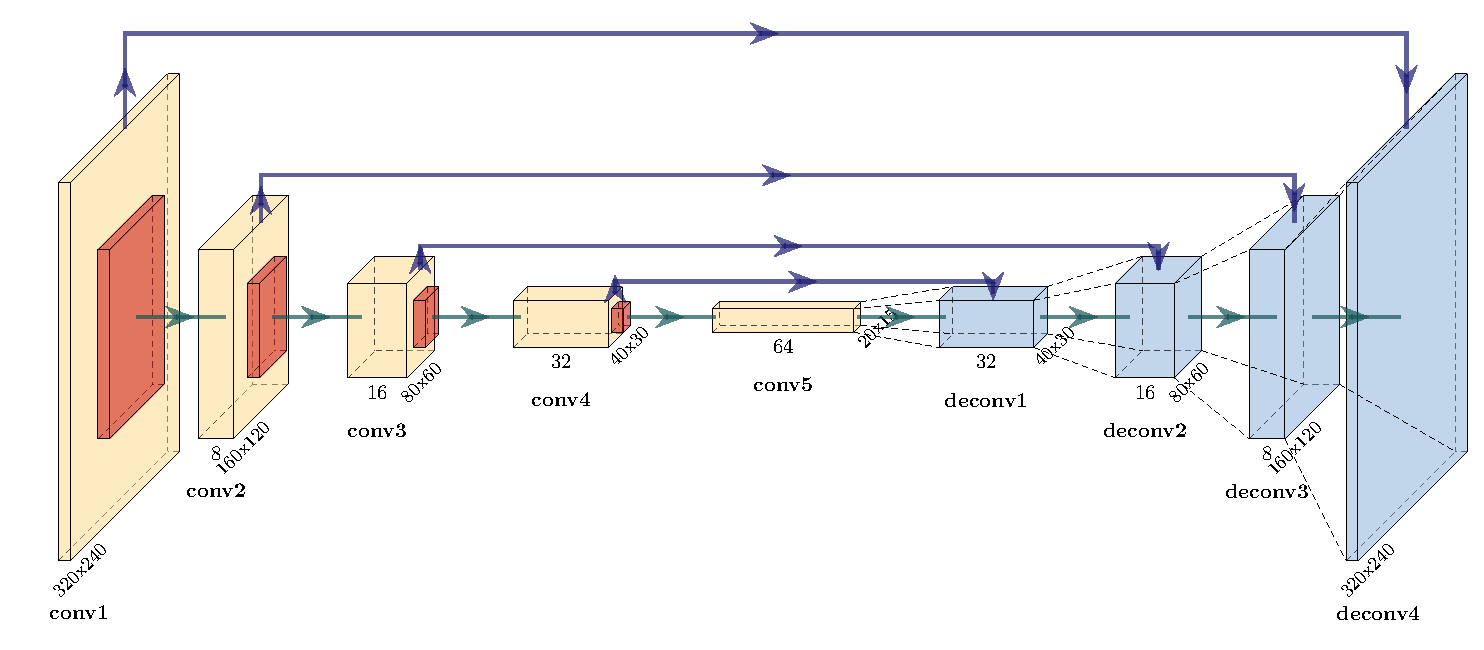
\includegraphics[width=0.9\textwidth]{images/models/unet}
  \caption{Neural network architecture of the U-Net. Created using PlotNeuralNet \citep{iqbal_harisiqbal88plotneuralnet_2018}.}
  \label{fig:unet_architecture}
\end{figure}

We chose to evaluate this architecture because it combines the denoising features of a traditional autoencoder with the ability to generate finer textures due to its skip connections. \citet{osin_fast_2018} utilise a modified U-Net to perform semantic segmentation on thermal multispectral images. Similar to the traditional autoencoder, the U-Net was trained for 100 epochs on the same dataset. 

Figure \ref{fig:autoencoder_pony_train_unet} displays the predicted LWIR image for the pony from the training dataset. Unlike the autoencoder, the U-Net is able to accurately represent the texture of the animal in the LWIR waveband.

\subsubsection{Results on unknown data}

After successful training of the networks, two images of ponies were retrieved from Wikimedia Commons. They were then fed into the network in an attempt to generate the corresponding LWIR images. The respective outputs can be seen in Figure \ref{fig:autoencoder_pony}.

\begin{figure}[ht]
  \centering
  \begin{subfigure}[h!]{0.22\textwidth}
    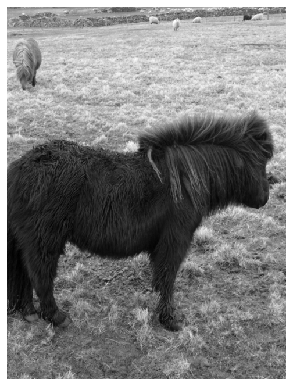
\includegraphics[width=\textwidth]{images/autoencoder/pony_1/gray.png}
    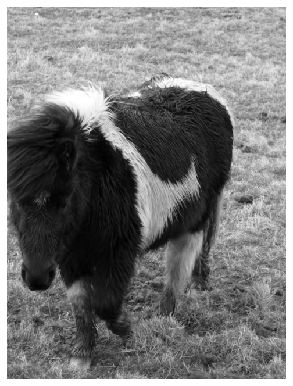
\includegraphics[width=\textwidth]{images/autoencoder/pony_2/gray.png}
    \caption{Original images}
  \end{subfigure}
  \begin{subfigure}[h!]{0.22\textwidth}
    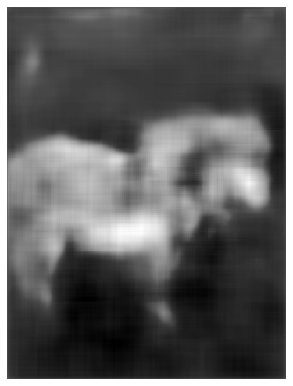
\includegraphics[width=\textwidth]{images/autoencoder/pony_1/auto.png}
    \includegraphics[width=\textwidth]{images/autoencoder/pony_2/auto.png}
    \caption{Autoencoder prediction}
  \end{subfigure}
  \begin{subfigure}[h!]{0.22\textwidth}
    \includegraphics[width=\textwidth]{images/autoencoder/pony_1/unet.png}
    \includegraphics[width=\textwidth]{images/autoencoder/pony_2/unet.png}
    \caption{U-Net prediction}
  \end{subfigure}
  \caption{Predicted LWIR signature of images of shetland ponies. Original images: "Shetland ponies at Sandwick" by Andrew Gray under CC BY-SA 2.0. URLs in List \ref{list:image_sources}.}
  \label{fig:autoencoder_pony}
\end{figure}

It appears as if the traditional autoencoder is more successful at generating LWIR images with plausible shapes than the U-Net. Various artefacts can be spotted in the U-Net image. Overall, the shape of the pony is not accurately represented. The U-Net is likely more overfitted on the training data.

Upon inspection of the bottom image, it can be seen that the white patch of the pony is also apparent in the autoencoder prediction. We conclude that the model is overfitted on dark ponies and is, therefore, unable to detect the patch as a normal part of the animal. Nonetheless, it seems possible that the autoencoder prediction might be accurate enough to be able to generate additional training data for a classifier.

%----------------------------------------------------------------------------------------------------------------------------------


\section{Mobile application}

Figure \ref{fig:app_uml} shows the architecture of the mobile application. The required components were implemented in a modular, extendable framework. The \lstinline{MainActivity} displays a list of all discovered FLIR cameras, including emulators. Each list item is represented by an instance of \lstinline{CameraArrayAdapter} and allows the user to start a \lstinline{CameraActivity} or \lstinline{ClassifierActivity} for the given sensor. 

\begin{figure}[ht]
  \centering
  \includegraphics[width=0.8\textwidth, trim={2.5cm 4.5cm 2.5cm 4.5cm}, clip=true]{images/app/App_UML}
  \caption{Simplified UML class diagram of the mobile application.}
  \label{fig:app_uml}
\end{figure}

Both activities share common functionality by extending \lstinline{AbstractCameraActivity}. This includes the \lstinline{CameraHandler}, which is responsible for communicating with the FLIR device and receiving a stream of images from the sensor. Furthermore, the \lstinline{AffineTransformer} initialises the OpenCV backend and provides functionality to perform affine transformations on images.

The \lstinline{CameraActivity} is designed to enable users to capture multispectral datasets. It contains a button for starting and stopping a recording. In addition, it uses an instance of the \lstinline{ImageWriter} class to save the captured frames to device storage and add them to the gallery.

Finally, the \lstinline{ClassifierActivity} initialises an instance of \lstinline{ModelHandler}. This class loads the TensorFlow Lite model and the class labels and performs real-time predictions on the images provided by the \lstinline{CameraHandler}. Screenshots of the complete application are attached in Figure \ref{fig:app_activities}.



%==================================================================================================================================

\chapter{Evaluation}
\label{evaluation}

To evaluate whether the addition of LWIR data can improve the performance of image classifiers on our dataset, we resorted to an evaluation comprising of three stages. Firstly, in Section \ref{eval_strategies}, we assessed the effectiveness of the model-invariant regularisation strategies we developed. Secondly, in Section \ref{eval_arch}, the relative accuracy of the proposed models and configurations was evaluated. Finally, we performed an in-depth analysis of the model with the highest performance in Section \ref{eval_final} and compared it to the pre-defined baselines.

\section{Training strategies}
\label{eval_strategies}

\subsection{Training-validation split}
\label{eval_train_val_split}

At first, the whole animals dataset was divided into training and validation data using stratified sampling and a validation split of $20\%$. When fitting the custom ResNet in late fusion mode using this split, near-perfect training and validation accuracy was achieved, as can be seen in Figure \ref{fig:acc_stratified}.  

\begin{figure}[ht]
  \centering
    \includegraphics[width=0.4\textwidth]{images/evaluation/stratified/accuracy}
  \caption{Training and validation accuracy over training epochs using a stratified train-validation split. The model achieves near-perfect validation accuracy using this strategy.}
  \label{fig:acc_stratified}
\end{figure}

This result is most likely due to the similarity of many images within individual subsets, as explained in Section \ref{classes_samples}. Since training and validation samples are drawn from the same raw dataset, it is likely that each subset is represented in both groups. Therefore, we conclude that it is likely that the model is significantly overfitted on the captured data and that the validation accuracy is not representative of the classifier's performance on chaotic new data. 

Fitting the model on the training dataset as defined in Section \ref{classes_samples}, validation scores dropped significantly. This was in accordance with our expectations, as the samples from the training and validation datasets are mostly independent. Therefore, the model is not able to overfit on the whole dataset anymore, and the validation score is more representative of the potential performance on new data.

\subsection{Data augmentation}

\subsubsection{Affine transformation}

The data augmentation strategy, as described in Section \ref{augmentation_impl} was evaluated by applying the augmentation script to the training dataset twice, with a multiplication factor of 2 and 5 respectively. The augmented datasets, thus, contain around 2 and 5 times as many samples than the original dataset. Furthermore, the class imbalances were equalised by the script by creating more samples of the underrepresented classes.

The custom ResNet in fusion mode was trained on the original and the two augmented datasets for 80 epochs. The complete classification reports can be inspected in Appendix \ref{appendix_augmentation}. The overall f1-score increased from $0.73$ without any augmentation to $0.78$ with augmentation with a factor of 2. For the factor-5-dataset, a slight increase of the f1-score to $0.79$ was determined. 

As creating even more augmented samples (factor 10) did not seem to significantly change the achieved accuracy, we decided to perform further evaluations with the factor-5-dataset.

\subsubsection{Generation of artificial data}

We used the autoencoder from Section \ref{autoencoder_implementation} to predict the LWIR signatures of ten images retrieved from Wikimedia Commons (sources in List \ref{list:image_sources}). We then selected a subset of our training dataset, containing images of the \textit{pony}, \textit{alpaca} and \textit{chicken} classes. A second copy of this dataset was created, and the ten predicted images were appended to the \textit{pony} class.

The custom ResNet in late fusion configuration was trained on both datasets. The full classification scores can be inspected in Appendices \ref{table:auto_scores_normal} and \ref{table:auto_scores_auto}. 

\begin{figure}[ht]
  \centering
  \begin{subfigure}[h!]{0.3\textwidth}
    \includegraphics[width=\textwidth]{images/evaluation/autoencoder/confusion_normal}
    \caption{Without generated images.}
    \label{fig:auto_confusion_normal}
  \end{subfigure}
  \begin{subfigure}[h!]{0.3\textwidth}
    \includegraphics[width=\textwidth]{images/evaluation/autoencoder/confusion_autoencoder}
    \caption{With generated images.}
    \label{fig:auto_confusion_auto}
  \end{subfigure}
  \caption{Confusion matrix of the custom ResNet in late fusion configuration on a simplified training dataset including and excluding artificially generated samples.}
  \label{fig:auto_confusion}
\end{figure}

The confusion matrices in Figure \ref{fig:auto_confusion} show that the amount of correctly classified ponies has indeed increased after including the artificially generated samples. However, more chicken and alpacas are mistakenly classified as ponies. The recall of the \textit{pony} class improved from $0.80$ to $0.87$, while the precision dropped from $0.73$ to $0.69$. The weighted average f1-score across the dataset remains unchanged at $0.82$. 

This behaviour can possibly be explained by the altered class balance of the dataset. As more samples of the \textit{pony} class are available in the training data, the model might simply have developed a stronger bias towards that class. As we could not reach a decisive conclusion about the effect of the incorporation of artificial data, we did not incorporate this approach into our further evaluation.

%----------------------------------------------------------------------------------------------------------------------------------

\section{Network architecture and configuration}
\label{eval_arch}

\subsection{Experimental setup}

To determine the multispectral configuration with the best performance out of all proposed models, we ran a grid search, as described in Section \ref{gridsearch_impl}. All models were trained for 80 epochs with a batch size of 32 samples, using the Adam optimiser with a learning rate of $10^{-6}$. 

The combination of batch size and learning rate was previously determined as an appropriate compromise between fast convergence and stability of the loss function. Generally, smaller batch sizes result in the training loss converging in fewer epochs, while larger batch sizes offer better computational efficiency due to parallelisability \citep{devarakonda_adabatch_2018}. 

Furthermore, smaller batch sizes make the training process more stochastic. More steps are taken during training. However, the smaller amount of samples per batch means that steps are less likely to be in the direction of the global minimum. On the other hand, it is more likely that the model can avoid getting stuck in local minima.

The effect of varying batch sizes is highly dependent on the specific properties of the dataset, optimiser and model. Whereas \citet{masters_revisiting_2018} achieved better generalisability on the CIFAR-10 dataset \citep{krizhevsky_learning_2009} using ResNet with smaller batch sizes, \citet{radiuk_impact_2017} reported higher testing accuracies on the same data using LeNet \citep{lecun_gradient-based_1998} with larger batch sizes. Our evaluation yielded an optimal batch size of 32 for the custom ResNet. The detailed results are shown in Figure \ref{fig:batch_size}.

Adam was published by \citet{kingma_adam_2014} and is generally considered to yield robust performance for deep learning algorithms \citep{alom_history_2018}.

\subsection{Grid search results}

The complete loss and accuracy history of all models and configurations are shown in Appendix \ref{appendix_grid_search}. Overall, the custom CNN achieved the lowest performance out of the three models. This is unsurprising, given the small number of trainable parameters compared to the other two models.

The custom ResNet implementation achieved the highest accuracy among the three models. The results for the ResNet can be seen in Figure \ref{fig:resnet_configs}. For all configurations, some overfitting can be observed, as the training losses and accuracies converge at near-perfect values. Moreover, we observe that, for most configurations, the validation loss initially drops faster than training loss. This is likely a result of the dropout layers, which are applied only when training.

\begin{figure}[ht]
  \centering
  \includegraphics[width=0.9\textwidth]{images/evaluation/gridsearch/ResNet}
  \caption{Cross-entropy loss and accuracy of different configurations of the ResNet implementation. The late fusion network achieves the highest validation accuracy.}
  \label{fig:resnet_configs}
\end{figure}

The LWIR-only configuration appears to be the least effective overall. It is possible that the lack of detailed textural information in the LWIR images makes it harder for the classifier to make a distinction between the different classes of animals.

The early fusion (\textit{stacked}) and score-level fusion (\textit{voting}) models achieve a validation accuracy similar to the RGB-only model. However, the validation loss of the early fusion classifier is converging towards that of the LWIR-only one.

Among all configurations, the late fusion (\textit{fusion}) model achieved the highest accuracy. Furthermore, the cross-entropy loss is comparatively low. This result confirms our theory that late-fusion-based approach proposed by \citet{wagner_multispectral_2016} can be applied to our multi-class classification problem. We selected this configuration as our final classifier due to its superior validation accuracy. 

%----------------------------------------------------------------------------------------------------------------------------------

\section{Final classifier}
\label{eval_final}

To obtain reliable scores for the selected model, we ran a 10-fold cross-validation on the late fusion ResNet and averaged the results. Since the validation dataset had to be kept entirely separate from the training dataset, as discussed in Section \ref{eval_train_val_split}, the k-fold split was performed only on the training dataset. During each fold, the non-selected samples were discarded instead of being used for validation.

Table \ref{table:final_classifier_scores} shows the precision, recall and f1-score of each class. The classes with the highest f1-score are \textit{goose}, \textit{cat} and \textit{hamburg chicken}. The classes with the lowest f1-score are and \textit{pony} and \textit{muscovy duck}. The pony class stands out with particularly low recall. Only half of all pony samples were classified as such.

\begin{table}[ht]
  \centering
  \begin{tabular}{@{}lllll@{}}
  \toprule
                        & \textbf{precision} & \textbf{recall} & \textbf{f1-score} &  \\ \midrule
  Cat                   & 0.87               & 1.00            & 0.93              &  \\
  Pony                  & 0.74               & 0.49            & 0.59              &  \\
  Hamburg chicken       & 0.91               & 0.88            & 0.90              &  \\
  Alpaca                & 0.98               & 0.67            & 0.79              &  \\
  Muscovy Duck          & 0.57               & 0.86            & 0.69              &  \\
  Chicken               & 0.64               & 0.85            & 0.73              &  \\
  Silkie Chicken        & 1.00               & 0.59            & 0.74              &  \\
  Goose                 & 0.96               & 1.00            & 0.98              &  \\
  \midrule
  \textbf{Weighted avg} & \textbf{0.83}      & \textbf{0.80}   & \textbf{0.80}     &  \\ \bottomrule
  \end{tabular}
  \caption{Precision, recall and f1-score of the final late fusion ResNet model.}
  \label{table:final_classifier_scores}
\end{table}

The chicken and muscovy duck classes suffer especially from low precision. This means that many samples are wrongly classified as those classes. A possible explanation for this is the wide variety of environments within the chicken and muscovy duck datasets. As outlined in Table \ref{table:train_test_dataset}, the amount of subsets used for the training dataset is the highest for both classes. It is likely that the model is biased in favour of these classes due to the great variety of backgrounds. 

From the confusion matrix in Figure \ref{fig:confusion}, it can be seen that there is some degree of confusion between similar classes, such as \textit{alpaca} and \textit{pony}, or \textit{silkie chicken} and \textit{muscovy duck}. The \textit{chicken} class is an exception to this rule, reinforcing the theory that the model is biased towards this class.

\subsection{t-SNE}
\label{tsne}

To further analyse these findings, we made use of t-distributed stochastic neighbour embedding (t-SNE), which was first introduced by \citet{maaten_visualizing_2008}. t-SNE is a dimensionality reduction technique for the visualisation of high-dimensional data. By flattening each image into a single vector, we obtain high-dimensional data points that t-SNE can be applied to. The result is a 2-D representation of the images that can be easily plotted and inspected. The same process can be applied to the outputs of the layers of the neural network.

Figure \ref{fig:test_tsne} shows the result of applying t-SNE to the validation dataset. In all four visualisations, most samples are concentrated in small clusters. These clusters most likely correspond to the subsets of the validation dataset. Images that were captured in quick temporal succession are likely to be nearly identical, which is why they are close together in the t-SNE visualisation. Figure \ref{fig:test_tsne_fc} demonstrates that, overall, the network successfully separates the samples into distinct classes.

\begin{figure}[ht]
  \centering
  \begin{subfigure}[h!]{0.4\textwidth}
    \includegraphics[width=\textwidth, trim={1cm 1cm 1cm 1cm}, clip]{images/evaluation/embedding/val/input}
    \caption{Input image.}
    \label{fig:test_tsne_input}
  \end{subfigure}
  \quad
  \begin{subfigure}[h!]{0.4\textwidth}
    \includegraphics[width=\textwidth, trim={1cm 1cm 1cm 1cm}, clip]{images/evaluation/embedding/val/vis}
    \caption{Output of final conv layer of VIS branch.}
    \label{fig:test_tsne_vis}
  \end{subfigure}

  \begin{subfigure}[h!]{0.4\textwidth}
    \includegraphics[width=\textwidth, trim={1cm 1cm 1cm 1cm}, clip]{images/evaluation/embedding/val/lwir}
    \caption{Output of final conv layer of LWIR branch.}
    \label{fig:test_tsne_lwir}
  \end{subfigure}
  \quad
  \begin{subfigure}[h!]{0.4\textwidth}
    \includegraphics[width=\textwidth, trim={1cm 1cm 1cm 1cm}, clip]{images/evaluation/embedding/val/fc}
    \caption{Output of final fully-connected layer.}
    \label{fig:test_tsne_fc}
  \end{subfigure}
  \caption{t-SNE visualisation of the validation dataset. As the features progress through the layers of the neural network, the classes become more easily separable.}
  \label{fig:test_tsne}
\end{figure}

As can be seen in Figure \ref{fig:test_tsne_input}, the cat images clearly stand out from the other classes even before being fed into the model. This is most likely a result of the fact that the cat images are the only ones that were captured in an indoor setting, resulting in a significantly lower illumination level.

This interpretation is further supported by the observation that the strict separation of the cat cluster persists throughout the VIS branch of the network, as shown in \ref{fig:test_tsne_vis}. The LWIR band, however, is not sensitive to illumination. Therefore, the LWIR branch of the network is unable to use the overall brightness of the image to make inferences about the classes. This explains why the distinctive cat cluster is not visible in Figure \ref{fig:test_tsne_lwir}.

A similar effect can be observed for the \textit{Hamburg chicken} class. A large Hamburg chicken cluster stands out in the t-SNE of the input image as well as the final convolutional layers of the VIS and LWIR branches. A likely explanation for this phenomenon is that many images of Hamburg chicken are partly occluded by a grid. Since this is unique to this class, it can be assumed that the model uses the grid as a feature to identify Hamburg chicken, resulting in undesirable background-related bias.

The \textit{alpaca} class demonstrates the effectiveness of the late fusion approach. Neither the VIS nor the LWIR branch are able to completely isolate and group together the alpaca images. However, the fully-connected part of the network is able to interpret the merged output features returned by the convolutional branches and accurately distinguish the class.

\subsection{Saliency analysis}

Saliency maps were first introduced by \citet{itti_model_1998} as a means of representing the conspicuity of every spatial location in an image. \citet{simonyan_deep_2014} developed this concept into class-specific saliency maps by using back-propagation of a classification.

Gradient-weighted Class Activation Mapping (Grad-CAM) is a novel visualisation technique developed by \citet{selvaraju_grad-cam_2020}. It uses the gradients of a target class at the last convolutional layer of a network to generate a heatmap showing the most important regions for the classification of that class.

Since the late fusion configuration of our ResNet has two parallel final convolutional layers, the gradient has to be computed for both layers. Figure \ref{fig:grad_cam} displays the Grad-CAM visualisation of four example images.

\begin{figure}[ht]
  \centering
  \begin{subfigure}[h!]{0.45\textwidth}
    \includegraphics[width=\textwidth]{images/evaluation/grad_cam/pos}
    \caption{Desirable example for both channels.}
    \label{fig:grad_cam_pos}
  \end{subfigure}
  \quad
  \begin{subfigure}[h!]{0.45\textwidth}
    \includegraphics[width=\textwidth]{images/evaluation/grad_cam/neg}
    \caption{Undesirable example for both channels.}
    \label{fig:grad_cam_neg}
  \end{subfigure}

  \begin{subfigure}[h!]{0.45\textwidth}
    \includegraphics[width=\textwidth]{images/evaluation/grad_cam/vis}
    \caption{Desirable VIS example.}
    \label{fig:grad_cam_vis}
  \end{subfigure}
  \quad
  \begin{subfigure}[h!]{0.45\textwidth}
    \includegraphics[width=\textwidth]{images/evaluation/grad_cam/lwir}
    \caption{Desirable LWIR example.}
    \label{fig:grad_cam_lwir}
  \end{subfigure}
  \caption{Grad-CAM visualisation of four example images. Warmer colours correspond to more attention by the last convolutional layer of the network. The left hand images in each pair represent the VIS images and corresponding heatmaps. The LWIR image and heatmap can be seen in the right hand images in each pair.}
  \label{fig:grad_cam}
\end{figure}

Figure \ref{fig:grad_cam_pos} shows a desirable example. Both final convolutional layers of the network focus on the head and feet of the alpaca to identify the class. This implies high generalisability even for images in different environments.

However, the network does not always focus on the desired relevant parts of the images. In the example shown in Figure \ref{fig:grad_cam_neg}, both the VIS and LWIR branches of the network do not focus on the muscovy duck. Instead, attention is directed towards the environment, such as the grass texture. It is unlikely that the network will be able to predict similar images with a different background.

The remaining two subfigures display examples where only either the VIS or LWIR branches of the network focus on the animals. These cases demonstrate an advantage of the multi-branch approach. The network performs better overall, as it can rely on the features of two semi-redundant branches.


\subsection{Accuracy at different lighting conditions}

As discussed in Section \ref{modality}, the modality difference between VIS and LWIR images suggests that thermal imaging systems should perform better in low-light conditions compared to visible-light-only systems.

To evaluate the relationship between classification performance and illumination, we calculated the mean and standard deviation of all pixel values of each image in the validation dataset. We then determined the cross-entropy loss of each prediction by the VIS-only, LWIR-only and late fusion ResNets and plotted it as a function of mean and standard deviation. The results are shown in Figure \ref{fig:illumination}.

\begin{figure}[ht]
  \centering
  \includegraphics[width=0.9\textwidth]{images/evaluation/illumination}
  \caption{Cross-entropy loss as a function of intensity mean and std of VIS and LWIR images in the validation dataset. The data has been smoothened with a running mean to emphasise general trends.}
  \label{fig:illumination}
\end{figure}

The overall result defies the expected behaviour of the models. It can be seen that the LWIR-only network performs significantly worse than its VIS-only and late fusion counterparts on low-light images. This further supports the theory we formulated in Section \ref{tsne}. The LWIR-only network likely uses the darkness of the cat images as a biased feature of the cat class, giving it near-perfect performance.

Since the LWIR band is not sensitive to illumination, the cat pictures do not generally stand out compared to in the VIS images. To obtain more robust results, a dataset with more well-balanced illumination levels would have to be acquired. Furthermore, the LWIR-only network has a high loss on samples with low LWIR mean intensity. A possible explanation for this is the lack of visible features in these images. 

\subsection{Comparison against the baseline}

As shown in Figure \ref{fig:resnet_configs}, the final late fusion model outperforms the visible-light-only baseline. Validation accuracy converges after around 50 epochs and remains stable. The final f1-score of $80\%$ is a significant improvement over the $74\%$ achieved by the VIS-only network. We, therefore, conclude that the use of a late fusion multispectral architecture can be beneficial for the performance of an image classifier.

To put these results into a relevant context, we compared the final classifier to a second, state-of-the-art VIS-only baseline. This model is an instance of ResNet152 v2 that has been pre-trained on the ImageNet dataset and transfer-trained on our dataset, as described in Section \ref{transfer_learning}.

The full training history is shown in Figure \ref{fig:baseline_configs}. The transfer-learned VIS-only classifier achieved a final f1-score of $92\%$, significantly outperforming our best model. Our attempts to create a late fusion model that has been pre-trained using the ImageNet data for the VIS branch and the FLIR dataset for the LWIR branch did not improve this baseline. The final f1-score of the transfer learned late fusion model remains unchanged compared to the VIS-only model at $0.92$.

Since larger training datasets usually result in more generalisable models and ImageNet contains over a million annotated samples, this result is unsurprising. As our late fusion model significantly outperformed the VIS-only variant when trained from scratch on the same data, we deem it likely that the pre-trained VIS-only baseline could be beaten given a large enough dataset.


%----------------------------------------------------------------------------------------------------------------------------------

\section{Mobile application deployment}

\subsection{Functionality validation}

To verify whether the deployment of the model to the mobile application is functional, a live evaluation on the actual animals was planned. The intention was to point the phone with the FLIR camera at the objects to evaluate the quality of the predictions. Since unforeseen circumstances emerged as a result of the SARS-CoV-2 epidemic, this evaluation could not be performed.

Instead, we qualitatively evaluated the deployment of the final model by pointing the phone and sensor at pictures from the existing validation dataset. Figure \ref{fig:app_screenshots} shows screenshots of the mobile application during this evaluation. A sample image was drawn from each class. Out of all eight images, the app gave six correct predictions.

It can, therefore, be concluded that the model is working correctly in the mobile application. Due to the physical limitations of the evaluation, the thermal channel could not be taken into consideration by the model, making the predictions less accurate. Furthermore, we observed a strong fluctuation of the predicted probabilities over time.

\begin{figure}[ht]
  \centering
  \begin{subfigure}[h!]{0.3\textwidth}
    \includegraphics[width=\textwidth, trim={0cm, 22cm, 0cm, 0cm}, clip]{images/app/screenshot_0.jpg}
  \end{subfigure}
  \begin{subfigure}[h!]{0.3\textwidth}
    \includegraphics[width=\textwidth, trim={0cm, 22cm, 0cm, 0cm}, clip]{images/app/screenshot_1.jpg}
  \end{subfigure}
  \begin{subfigure}[h!]{0.3\textwidth}
    \includegraphics[width=\textwidth, trim={0cm, 22cm, 0cm, 0cm}, clip]{images/app/screenshot_2.jpg}
  \end{subfigure}
  \caption{Screenshots of the mobile application's predictions with the late fusion model. The top predictions display the correct classes. Due to exceptional circumstances, only pictures of animals could be evaluated instead of the animals themselves.}
  \label{fig:app_screenshots}
\end{figure}

\subsection{Performance, latency and battery usage}

The application was installed on a OnePlus 7 Android device to evaluate the latency of real-time classification. TensorFlow Lite was configured to use the device's GPU for predictions. The RGB-only and feature-level fusion configurations of the custom ResNet were evaluated by running the application in classification mode and performing 1000 predictions. As visible in Figure \ref{fig:app_screenshots}, the application displays the mean and standard deviation of classification times since launch. The following values are readings from this output.

Whereas the RGB-only model took an average of $40.99 ms$, $\sigma = 4.55 ms$ for a single prediction, the late fusion model performed a prediction every $70.24 ms$, $\sigma = 6.79 ms$. This equates to $14.24$ predictions per second, which is significantly higher than the sensor frame rate of $8.7 Hz$. 
Infrequent stuttering of the image feed in both the camera and classifier activities are a result of the sensor occasionally closing the shutter and automatically recalibrating, as outlined in the user guide\footnote{\url{http://www.flirmedia.com/flir-one/flir-one-pro/user-guides/flir-one-pro-user-guide.html}}.

Finally, the battery impact of running the application was evaluated by running the classifier activity for 20 minutes. No other applications were active on the device simultaneously. According to Android's battery usage statistics (Figure \ref{fig:app_battery}), our application used around $8\%$ of the device's $3700 mAh$ battery capacity over the course of the $20 min$. This implies a theoretical maximum usage time of $4.17 h$, assuming the usage statistics are accurate. Based on the results of this evaluation, we conclude that the multispectral model is suitable for real-time classification tasks on edge devices.

%==================================================================================================================================
\chapter{Conclusion}

\section{Summary}

This dissertation explored the benefits and drawbacks of multispectral image classification with a thermal and visible-light camera. A classifier based on the ResNet deep learning architecture was developed, achieving a validation f1-score of $80\%$.

Our evaluation demonstrates that a model based on late fusion of the thermal and visible-light features, similar to \citet{wagner_multispectral_2016}, clearly outperforms the VIS-only baseline. This is the case even in settings with sufficient illumination.

The classifier has been successfully deployed to a mobile edge device and can be run in real-time with tolerable latency. This demonstrates the suitability of the system for mobile environments with low computational power, such as phones and self-driving cars.

However, our model was not able to beat the second proposed baseline of a state-of-the-art VIS-only classifier that was pre-trained on the ImageNet dataset. Attempts to perform transfer learning on an LWIR classifier did not manage to improve our model's performance. We conclude that the lack of available thermal datasets remains a significant problem for the development of LWIR-based computer vision systems.

Furthermore, our t-SNE and saliency analysis of the final model reveals problems with background-related bias. These issues are likely a result of a noisy and insufficiently diverse dataset. 

Nonetheless, our evaluation suggests that our multi-branch network architecture increases the system's robustness by providing more redundant features (XXX rephrase). We conclude that thermal multispectral imaging can significantly improve the performance of deep learning models for the recognition of animals.

%----------------------------------------------------------------------------------------------------------------------------------

\section{Future work}

We attempted to increase the generalisability of our classifier by generating artificial LWIR data using a convolutional autoencoder. Since the scale of this experiment was limited, no reliable conclusion about the effectiveness of this strategy could be drawn. To further evaluate the feasibility of incorporating artificially generated data into the training process, a generative adversarial network could be designed and applied to a sufficiently large visible-light dataset.

Moreover, many generalisation problems of our model are likely a result of poorly framed input images. Furthermore, the framing of objects is likely to be noisy when using the mobile application. A more robust approach for this usage scenario could involve the development of an object detection model. Such a model would support the detection of multiple objects in a single image at varying distances and positions. State-of-the-art architectures such as YOLO \citep{redmon_you_2016, redmon_yolov3_2018} promise low inference times and might be suitable for this task. 

Our review of existing image registration metrics concluded that the problem of quantifying the alignment of VIS and LWIR images has not yet been conclusively solved. Further investigation into robust registration metrics for thermal and visible-light images might be necessary to accelerate future research into the benefits and drawbacks of thermal multispectral imaging.

Finally, for applications involving a continuous video feed, such as the mobile application, video surveillance systems or self-driving cars, additional robustness could be added to the model by processing sequences of data instead of single images. Promising approaches for this problem include deep recurrent neural networks and long short-term memory (LSTM) architectures \citep{hochreiter_long_1997}.

%==================================================================================================================================
%
% 
%==================================================================================================================================
%  APPENDICES  

\begin{appendices}

%==================================================================================================================================

\chapter{Multispectral CNN configurations}
\label{appendix_arch}

\begin{figure}[ht]
  \centering
  \includegraphics[width=0.25\textwidth]{images/models/keras/stacked.png}
  \caption{Architecture of AlexNet in stacked configuration.}
\end{figure}

\begin{figure}[ht]
  \centering
  \includegraphics[width=0.6\textwidth]{images/models/keras/voting.png}
  \caption{Architecture of AlexNet in voting configuration.}
\end{figure}

\begin{figure}[ht]
  \centering
  \includegraphics[width=0.6\textwidth]{images/models/keras/fusion.png}
  \caption{Architecture of AlexNet in late fusion configuration.}
\end{figure}

%==================================================================================================================================

\chapter{Data augmentation evaluation}
\label{appendix_augmentation}

\begin{table}[H]
  \centering
  \begin{tabular}{@{}lllll@{}}
  \toprule
                        & \textbf{precision} & \textbf{recall} & \textbf{f1-score} &  \\ \midrule
  Cat                   & 0.57               & 1.00            & 0.72              &  \\
  Pony                  & 0.83               & 0.60            & 0.70              &  \\
  Hamburg chicken       & 0.74               & 0.89            & 0.81              &  \\
  Alpaca                & 1.00               & 0.52            & 0.68              &  \\
  Muscovy Duck          & 0.59               & 0.65            & 0.62              &  \\
  Chicken               & 0.53               & 0.61            & 0.57              &  \\
  Silkie Chicken        & 1.00               & 0.60            & 0.75              &  \\
  Goose                 & 0.98               & 1.00            & 0.99              &  \\
  \midrule
  \textbf{Weighted avg} & \textbf{0.78}      & \textbf{0.73}   & \textbf{0.73}     &  \\ \bottomrule
  \end{tabular}
  \caption{Precision, recall and f1-score of the late fusion ResNet model without affine data augmentation.}
  \label{table:appendix_affine_1}
\end{table}

\begin{table}[H]
  \centering
  \begin{tabular}{@{}lllll@{}}
  \toprule
                        & \textbf{precision} & \textbf{recall} & \textbf{f1-score} &  \\ \midrule
  Cat                   & 0.70               & 1.00            & 0.82              &  \\
  Pony                  & 0.97               & 0.59            & 0.73              &  \\
  Hamburg chicken       & 0.96               & 0.86            & 0.91              &  \\
  Alpaca                & 1.00               & 0.63            & 0.77              &  \\
  Muscovy Duck          & 0.53               & 0.86            & 0.65              &  \\
  Chicken               & 0.61               & 0.74            & 0.67              &  \\
  Silkie Chicken        & 1.00               & 0.57            & 0.73              &  \\
  Goose                 & 1.00               & 1.00            & 1.00              &  \\
  \midrule
  \textbf{Weighted avg} & \textbf{0.84}      & \textbf{0.78}   & \textbf{0.78}     &  \\ \bottomrule
  \end{tabular}
  \caption{Precision, recall and f1-score of the late fusion ResNet model with affine data augmentation (factor 2).}
  \label{table:appendix_affine_2}
\end{table}

\begin{table}[H]
  \centering
  \begin{tabular}{@{}lllll@{}}
  \toprule
                        & \textbf{precision} & \textbf{recall} & \textbf{f1-score} &  \\ \midrule
  Cat                   & 0.89               & 1.00            & 0.94              &  \\
  Pony                  & 0.97               & 0.48            & 0.64              &  \\
  Hamburg chicken       & 1.00               & 0.79            & 0.88              &  \\
  Alpaca                & 0.97               & 0.74            & 0.84              &  \\
  Muscovy Duck          & 0.47               & 0.78            & 0.59              &  \\
  Chicken               & 0.61               & 0.84            & 0.70              &  \\
  Silkie Chicken        & 1.00               & 0.57            & 0.73              &  \\
  Goose                 & 1.00               & 1.00            & 1.00              &  \\
  \midrule
  \textbf{Weighted avg} & \textbf{0.85}      & \textbf{0.79}   & \textbf{0.79}     &  \\ \bottomrule
  \end{tabular}
  \caption{Precision, recall and f1-score of the late fusion ResNet model with affine data augmentation (factor 5).}
  \label{table:appendix_affine_3}
\end{table}

\begin{captionedList}
  \begin{enumerate}
    \item{\url{https://commons.wikimedia.org/wiki/File:Shetland_pony_in_the_snow,_Baltasound_-_geograph.org.uk_-_1691743.jpg}}
    \item{\url{https://commons.wikimedia.org/wiki/File:Sandwick_Shetland_Pony.jpg}}
    \item{\url{https://commons.wikimedia.org/wiki/File:Shetland_pony_(2).jpg}}
    \item{\url{https://commons.wikimedia.org/wiki/File:Grey_Shetland_pony_-_geograph.org.uk_-_1606748.jpg}}
    \item{\url{https://commons.wikimedia.org/wiki/File:Shetland_Ponies_and_Iron_Horse,_Huxter,_Whalsay,_Shetland_-_geograph.org.uk_-_145763.jpg}}
    \item{\url{https://commons.wikimedia.org/wiki/File:Shetland_ponies_at_Sandwick.jpg}}
    \item{\url{https://commons.wikimedia.org/wiki/File:Pony_at_Mosedale.jpg}}
    \item{\url{https://commons.wikimedia.org/wiki/File:Pony_on_Lund_beach_-_geograph.org.uk_-_1741711.jpg}}
    \item{\url{https://commons.wikimedia.org/wiki/File:Fell_ponies,_West_Fell.jpg}}
    \item{\url{https://commons.wikimedia.org/w/index.php?title=Special:Search&limit=20&offset=420&profile=default&search=shetland+pony&advancedSearch-current=%7B%7D&ns0=1&ns6=1&ns12=1&ns14=1&ns100=1&ns106=1#/media/File:Jielbeaumadier_cheval_5_scva_paris_2012.jpeg}}
  \end{enumerate}
  \caption{Image sources for the autoencoder. All images retrieved under CC BY-SA 2.0.}
  \label{list:image_sources}
\end{captionedList}

\begin{table}[H]
  \centering
  \begin{tabular}{@{}lllll@{}}
  \toprule
                        & \textbf{precision} & \textbf{recall} & \textbf{f1-score} &  \\ \midrule
  Pony                  & 0.73               & 0.80            & 0.77              &  \\
  Alpaca                & 1.00               & 0.60            & 0.75              &  \\
  Chicken               & 0.80               & 0.99            & 0.89              &  \\
  \midrule
  \textbf{Weighted avg} & \textbf{0.85}      & \textbf{0.82}   & \textbf{0.82}     &  \\ \bottomrule
  \end{tabular}
  \caption{Precision, recall and f1-score of the custom ResNet in late fusion configuration on the simplified dataset including artificially generated samples.}
  \label{table:auto_scores_normal}
\end{table}

\begin{table}[H]
  \centering
  \begin{tabular}{@{}lllll@{}}
  \toprule
                        & \textbf{precision} & \textbf{recall} & \textbf{f1-score} &  \\ \midrule
  Pony                  & 0.69               & 0.87            & 0.77              &  \\
  Alpaca                & 1.00               & 0.60            & 0.75              &  \\
  Chicken               & 0.84               & 0.97            & 0.90              &  \\
  \midrule
  \textbf{Weighted avg} & \textbf{0.86}      & \textbf{0.83}   & \textbf{0.82}     &  \\ \bottomrule
  \end{tabular}
  \caption{Precision, recall and f1-score of the custom ResNet in late fusion configuration on the simplified dataset including artificially generated samples.}
  \label{table:auto_scores_auto}
\end{table}

%==================================================================================================================================

\chapter{Batch size evaluation}
\label{appendix_batch_size}

\begin{figure}[ht]
  \centering
  \includegraphics[width=0.9\textwidth]{images/evaluation/batch_size/history}
  \caption{Cross-entropy loss and accuracy of the custom ResNet with varying batch sizes.}
  \label{fig:batch_size}
\end{figure}

%==================================================================================================================================

\chapter{Grid search results}
\label{appendix_grid_search}

\begin{figure}[ht]
  \centering
  \includegraphics[width=0.7\textwidth]{images/evaluation/gridsearch/comparison}
  \caption{Validation f1-score of all classifiers and all configurations.}
  \label{fig:gridsearch_bar}
\end{figure}

\begin{figure}[ht]
  \centering
  \includegraphics[width=0.9\textwidth]{images/evaluation/gridsearch/CustomNet}
  \caption{Cross-entropy loss and accuracy of different configurations of the custom net.}
  \label{fig:customnet_configs}
\end{figure}

\begin{figure}[ht]
  \centering
  \includegraphics[width=0.9\textwidth]{images/evaluation/gridsearch/AlexNet}
  \caption{Cross-entropy loss and accuracy of different configurations of the AlexNet implementation.}
  \label{fig:alexnet_configs}
\end{figure}

\begin{figure}[ht]
  \centering
  \includegraphics[width=0.9\textwidth]{images/evaluation/gridsearch/ResNet}
  \caption{Cross-entropy loss and accuracy of different configurations of the ResNet implementation.}
  \label{fig:resnet_configs_app}
\end{figure}

\chapter{Baseline}
\label{appendix_baseline}

\begin{figure}[ht]
  \centering
  \includegraphics[width=0.8\textwidth]{images/evaluation/baseline}
  \caption{Cross-entropy loss and accuracy of different configurations of the transfer learned baseline.}
  \label{fig:baseline_configs}
\end{figure}

%==================================================================================================================================

\chapter{Confusion matrix}

\begin{figure}[ht]
  \centering
  \includegraphics[width=0.8\textwidth]{images/evaluation/confusion/final}
  \caption{Confusion matrix of the final late fusion ResNet model.}
  \label{fig:confusion}
\end{figure}

%==================================================================================================================================

\chapter{Mobile application}

\begin{figure}[ht]
  \centering
  \begin{subfigure}[h!]{0.32\textwidth}
    \includegraphics[width=\textwidth]{images/app/overview.jpg}
    \caption{Home activity.}
    \label{fig:app_activities_home}
  \end{subfigure}
  \begin{subfigure}[h!]{0.32\textwidth}
    \includegraphics[width=\textwidth]{images/app/camera.jpg}
    \caption{Camera activity.}
    \label{fig:app_activities_camera}
  \end{subfigure}
  \begin{subfigure}[h!]{0.32\textwidth}
    \includegraphics[width=\textwidth]{images/app/screenshot_0.jpg}
    \caption{Classifier activity.}
    \label{fig:app_activities_classifier}
  \end{subfigure}
  \caption{Activities of the mobile application. From the home activity \subref{fig:app_activities_home}, users can launch camera or classifier mode for any discovered FLIR camera. The camera activity \subref{fig:app_activities_camera} can be used to capture thermal multispectral datasets. The classifier activity \subref{fig:app_activities_classifier} can be used for real-time multi-class classification.}
  \label{fig:app_activities}
\end{figure}

\begin{figure}[ht]
  \centering
  \includegraphics[width=0.4\textwidth, trim={0cm 32cm 0cm 0cm}, clip]{images/app/battery}
  \caption{Battery usage statistics of running the mobile application in classification mode for 20 minutes. The application reduced the battery charge by $8\%$ during the 20 minutes.}
  \label{fig:app_battery}
\end{figure}


\end{appendices}

%==================================================================================================================================
%   BIBLIOGRAPHY   

% The bibliography style is abbrvnat
% The bibliography always appears last, after the appendices.

\bibliographystyle{abbrvnat}

\bibliography{l4proj}

\end{document}
